
% MODELO LATEX PARA TCC DO IFCE 
% ELABORADO POR CARINA TEIXEIRA DE OLIVEIRA
% SETEMBRO DE 2017

\documentclass[
12pt, % tamanho da fonte
openright, % capítulos começam em pág ímpar (insere página vazia caso preciso)
oneside, % para impressão somente frente. Oposto a twoside (frente e verso)
a4paper, % tamanho do papel. 
% 	% -- opções do pacote babel --
english,% idioma adicional para hifenização
%french,% idioma adicional para hifenização
%spanish,% idioma adicional para hifenização
brazil,	% o último idioma é o principal do documento
]{abntex2}

% ------------------------
% PACOTES
% Mapear caracteres especiais no PDF
\usepackage{cmap}
% Usa a fonte Latin Modern
\usepackage{times}			
% Selecao de codigos de fonte.
\usepackage[T1]{fontenc}		
% Codificacao do documento (conversão automática dos acentos)
\usepackage[utf8]{inputenc}		
% Indenta o primeiro parágrafo de cada seção.
\usepackage{indentfirst}		
% Controle das cores
\usepackage{color}				
% Inclusão de gráficos
\usepackage{graphicx}			
\usepackage{multicol}
\usepackage{multirow}
%capitulos
\usepackage{titlesec}
% Pacotes adicionais, usados apenas no âmbito do Modelo Canônico do abnteX2
% para geração de dummy text
\usepackage{lipsum}				
% Pacotes de citações
% Paginas com as citações na bibl
\usepackage[brazilian,hyperpageref]{backref}	 
% Citações padrão ABNT
\usepackage[alf]{abntex2cite}	
% CONFIGURAÇÕES DE PACOTES
% Configurações do pacote backref
% Usado sem a opção hyperpageref de backref
\renewcommand{\backrefpagesname}{Citado na(s) página(s):~}
% Texto padrão antes do número das páginas
\renewcommand{\backref}{}
%Define os textos da citação
\renewcommand*{\backrefalt}[4]{
	\ifcase #1 %
		Nenhuma citação no texto.%
	\or
		Citado na página #2.%
	\else
		Citado #1 vezes nas páginas #2.%
	\fi}

% ------------------------
% atalhos
\titulo{UM GUIA DE BOAS PRÁTICAS PARA O DESENVOLVIMENTO DE APLICAÇÕES \textit{WEB} NO \textit{FRONT-END}}
\autor{IVOMAR DE ARRUDA SANTOS}
\local{ARACATI-CE}
\data{2018}
\instituicao{Instituto Federal de Educação, Ciência e Tecnologia do Ceará}
\tipotrabalho{Trabalho de Conclusão de Curso (TCC)}
% O preambulo deve conter o tipo do trabalho, o objetivo, o nome da instituição e a área de concentração 
\preambulo{Modelo canônico de Relatório Técnico e/ou Científico em conformidade
com as normas ABNT apresentado à comunidade de usuários \LaTeX.}


% ------------------------
% Configurações de aparência do PDF final
% alterando o aspecto da cor azul
\definecolor{blue}{RGB}{41,5,195}
%informações do PDF
\makeatletter
\hypersetup{
    %pagebackref=true,
	pdftitle={\@title}, 
	pdfauthor={\@author},
    pdfsubject={\imprimirpreambulo},
	pdfcreator={LaTeX with abnTeX2},
	%pdfkeywords={abnt}{latex}{abntex}{abntex2}{relatório técnico}, 
	colorlinks=true,% false: boxed links; true: colored links
    linkcolor=blue,	% color of internal links
    citecolor=blue,	% color of links to bibliography
    filecolor=magenta, % color of file links
	urlcolor=blue,
	bookmarksdepth=4
}
\makeatother

% -----------------------
% Usando o listings
\usepackage{listings}
% – inicio codigo fonte
\lstset{numbers=left,
stepnumber=1,
firstnumber=1,
numberstyle=\tiny,
extendedchars=true,
breaklines=true,
frame=tb,
basicstyle=\footnotesize,
stringstyle=\ttfamily,
showstringspaces=false
}

\renewcommand{\lstlistingname}{Código}
\renewcommand{\lstlistlistingname}{Lista de Listagens}
% – fim codigo fonte


% ------------------------
% Espaçamentos entre linhas e parágrafos 
% O tamanho do parágrafo é dado por:
\setlength{\parindent}{1.5cm}
% Controle do espaçamento entre um parágrafo e outro:
\setlength{\parskip}{0.2cm}  % tente também \onelineskip

% compila o indice
\makeindex
%\input{modeloCapitulos}

\begin{document}

%PARA UTILIZAR ARIAL
\fontfamily{phv}  %fonte Arial
\renewcommand{\rmdefault}{phv}      

% Retira espaço extra obsoleto entre as frases.
%\frenchspacing 
\thispagestyle{empty}
\vfill
\begin{center}

\begin{figure}[t]
\centering

\includegraphics[width=4cm]{figuras/ifce-ceara.png}%\\[-0.01in]
\end{figure}
\vspace{0.5 cm}
{\normalsize\bfseries INSTITUTO FEDERAL DE EDUCAÇÃO, CIÊNCIA E TECNOLOGIA DO CEARÁ} \\
{\normalsize\bfseries IFCE CAMPUS ARACATI} \\
{\normalsize\bfseries COORDENADORIA DE CIÊNCIA DA COMPUTAÇÃO}  \\ 
{\normalsize\bfseries BACHARELADO EM CIÊNCIA DA COMPUTAÇÃO}  \\ 

\vspace*{1in}
\begin{large} \bfseries \imprimirautor \end{large}\\[0.4in]

\vspace*{4cm}
\noindent \\
\large\bfseries \imprimirtitulo \\
\vfill
\normalsize\bfseries{\imprimirlocal\\\imprimirdata}

\end{center}
\normalsize
\vfill
\begin{center}

{\imprimirautor\\}
\vspace{3cm}
{\textsc \imprimirtitulo\\}
\vspace{5cm}
\hspace{.45\linewidth}
\begin{minipage}{.50\linewidth}
Trabalho de Conclusão de Curso (TCC) apresentado ao curso de Bacharelado em Ciência da Computação do Instituto Federal de Educação, Ciência e Tecnologia do Ceará - IFCE - Campus Aracati, como requisito parcial para obtenção do Título de Bacharel em Ciência da Computação.

\vspace{0.5 cm}

Orientador: Prof. Dr. Reinaldo Bezerra Braga

\end{minipage}

\vspace{2cm}
\vfill
{\large \imprimirlocal\\\imprimirdata}

\end{center}

\begin{fichacatalografica}
	\sffamily
	\vspace*{\fill}					% Posição vertical
	\begin{center}					% Minipage Centralizado
	\fbox{\begin{minipage}[c][8cm]{13.5cm}		% Largura
	\small
	\imprimirautor
	%Sobrenome, Nome do autor
	
	\hspace{0.5cm} \imprimirtitulo  / \imprimirautor. --
	\imprimirlocal, \imprimirdata-
	
	\hspace{0.5cm} \pageref{LastPage} p. : il. (algumas color.) ; 30 cm.\\
	
	\hspace{0.5cm} \imprimirorientadorRotulo~\imprimirorientador\\
	
	\hspace{0.5cm}
	\parbox[t]{\textwidth}{\imprimirtipotrabalho~--~\imprimirinstituicao,
	\imprimirdata.}\\
	
	\hspace{0.5cm}
		1. Palavra-chave1
		2. Palavra-chave2.
		2. Palavra-chave3.
% 		I. Emanuel Bezerra Rodrigues.
% 		II. Instituto Federal de Educação, Ciência e Tecnologia do Ceará - Campus Aracati.
% 		III. Coordenadoria de Ciência da Computação.
% 		IV. Título da dissertação			
	\end{minipage}}
	\end{center}
\end{fichacatalografica}
\begin{folhadeaprovacao}
\vfill
\begin{center}

{\imprimirautor\\}
\vspace{1.5cm}
{\textsc \imprimirtitulo\\}
\vspace{1.5cm}
\hspace{.45\linewidth}
\begin{minipage}{.50\linewidth}
Trabalho de Conclusão de Curso (TCC) apresentado ao curso de Bacharelado em Ciência da Computação do Instituto Federal de Educação, Ciência e Tecnologia do Ceará - IFCE - Campus Aracati, como requisito parcial para obtenção do Título de Bacharel em Ciência da Computação. 
\end{minipage}
\vspace{1.0 cm}

\end{center}

\noindent\\
{Aprovado em 18 de Abril de \imprimirdata}

\vspace{1.5 cm}
\begin{center}
{BANCA EXAMINADORA}
\assinatura{Prof. Dr. Reinaldo Bezerra Braga (Orientador) \\ 
Instituto Federal do Ceará (IFCE)}
\assinatura{Prof. Bsc. Thiago Felippe de Lima Bandeira (Co-orientador) \\ 
Instituto Federal do Ceará (IFCE)}
\assinatura{Profª. Dra. Carina Teixeira de Oliveira\\ 
Instituto Federal do Ceará (IFCE)}
\assinatura{Prof. Msc. Silas Santiago Lopes\\ 
Instituto Federal do Ceará (IFCE)}
\end{center}
\end{folhadeaprovacao}
\vfill
\begin{center}
{\textbf{DEDICATÓRIA}\\}
\end{center}

\noindent À minha persistência.\\
\noindent Ao meu orgulho.\\
\noindent Aos meus pais e especialmente irmãos. Também aos Amigos com A maiúsculo pela motivação e por serem pé no saco, obrigado!\\

Aos meus amigos que compartilham do meu empenho e sacrifício e que se mostraram presentes até mesmo quando busquei ausentar-me. Dedico-lhes o meu sucesso.

À minha esposa que não existe, minha filha que não nasceu e a toda minha família imaginária que, com muito carinho e apoio, não mediram esforços para que eu chegasse até esta etapa de minha vida.

Ao CS:GO e às pessoas com quem convivi nesses espaços ao longo desses anos. A experiência de uma produção compartilhada na comunhão com amigos nesses espaços foram a melhor experiência da minha formação acadêmica. Em especial ao meu clã, Berglândia, Grego e Cheira.\\
\vfill
\begin{center}
{\textbf{AGRADECIMENTOS}}
\end{center}

Ao LAR e IFCE pelo ambiente criativo e amigável que proporciona.

Ao Prof. Dr. Mauro Oliveira, pelo discurso no meu primeiro dia de aula, o que contribuiu para a minha permanência nesta instituição.

Ao Prof. Dr. Reinaldo Braga, pela orientação, apoio, confiança e principalmente pela amizade.

À Profª. Dra. Carina Teixeira, por ser implacável e motivacional, além de ser fundamentalmente inspiradora para a elaboração deste trabalho.

Ao Professor Thiago Bandeira, pelo suporte e pela dedicação no pouco tempo que lhe coube para auxiliar e co-orientar.

Aos professores, Silas, Felipe, Raquel, Alberto, Evandro, por terem deixado valores, algo mais importante que apenas a grade curricular.

A todos que direta ou indiretamente fizeram parte da minha formação profissional, o meu muito obrigado.
\vfill
\begin{center}
{\textbf{RESUMO}\\}
\end{center}
\noindent

Atualmente, é perceptível a crescente utilização e difusão dos serviços existentes na rede mundial de computadores, também conhecida pela sigla WWW (em inglês \textit{World Wide Web}) ou simplesmente \textit{Web}, que é um sistema de documentos interligados e que são aplicados na Internet. Sua arquitetura é dividida principalmente em duas partes interconectadas, chamadas de cliente e servidor. Neste modelo, as responsabilidades são repartidas e juntas garantem a execução de serviços e sistemas de redes. O lado servidor, como o nome explicita, é responsável por servir seus clientes, disponibilizando o serviço para responder a uma demanda do cliente. Por outro lado, o cliente requisita o serviço, ou seja, inicia a interação a partir de uma requisição do usuário, através de um navegador (\textit{browser}). Desta forma, o usuário pode realizar requisições de conteúdo dinâmico com o servidor, através de diversos protocolos de comunicação, sendo o HTTP (\textit{Hypertext Transfer Protocol}) o mais comum. Além disso, as tecnologias empregadas para o perfeito funcionamento de uma aplicação \textit{Web} também são subdivididas. É comum observar que, geralmente, toda interação visual está localizado no cliente. Já no servidor, localiza-se todo o serviço de armazenamento de dados e regras de negócio da aplicação \textit{Web}. Com isto, é sabido que o serviço rodando no lado cliente serve como interface direta com o utilizador. Consequentemente, sistemas mal estruturados e incompletos podem fornecer ao usuário uma péssima primeira impressão. Portanto, é responsabilidade do desenvolvedor garantir que erros não ocorram, tais como: Ausência de retorno visual das interações; Tratamento correto de dados e validações; Aparência da aplicação e incompatibilidade entre dispositivos. Em outras palavras, é importante evitar erros que impactam o funcionamento do sistema e geram desconforto para a usabilidade. Neste contexto, este trabalho apresenta boas práticas de desenvolvimento de serviços \textit{Web} e explora técnicas de otimização da experiência do usuário ao navegar através de aplicações \textit{Web}. São utilizados padrões definidos por entidades reguladoras (W3C) e grandes grupos atuantes (WHATWG).

\vspace{\onelineskip}
 \noindent
 \textbf{Palavras-chave}: Aplicações \textit{Web}; Desenvolvimento; Otimização.
\vfill
\begin{center}
{\textbf{ABSTRACT}\\}
\end{center}

\noindent

Nowadays, it’s noticeable the growing use and dissemination of existing services on the World Wide Web, also known by the acronym WWW or simply Web, which is a system of interconnected documents and that are applied on the Internet. Its architecture is divided mainly into two interconnected parts, called client and server. In this model, the responsibilities are shared and guarantee the execution of services and systems of networks. The server side, as the name explicitly, is responsible for serving its customers, making the service available to respond to a customer's demand. On the other hand, the client requests the service through a browser, initiating the interaction from a user request. In this way, the user can perform dynamic content requests with the server, through several communication protocols, being HTTP (Hypertext Transfer Protocol) the most common. In addition, the technologies employed for the perfect functioning of a Web application are also subdivided. It is common to note that, generally, every visual interaction is located on the client side. Even in the server side, it locates the service of data storage and business rules of the Web application.  Thus, it is known that the service running on the client side serves as a direct interface with the user. Consequently, poorly structured and incomplete systems can provide the user a poor first impression. Therefore, it is a developer’s responsibility ensure that errors do not occur, such as: absence of visual feedback of interactions; Correct treatment of data and validations; Appearance of the application and incompatibility between devices. In other words, it is important to avoid errors that impact the functioning of the system and generate discomfort for usability. In this context, this paper presents a set of good Web service development practices, exploring user experience optimization techniques during the use of Web applications. Standards defined by regulators (W3C) and large working groups (WHATWG) are used. 
 
 \vspace{\onelineskip}
    
 \noindent
 \textbf{Keywords}: Web Applications; Development; Optimization.

\vfill
\begin{center}
{\textbf{LISTA DE ILUSTRAÇÕES}}
\end{center}

\renewcommand\listfigurename{}
\listoffigures* % * indica que não aparecerá no sumário

\vfill
\begin{center}
{\textbf{LISTA DE TABELAS}}
\end{center}

\renewcommand\listtablename{}
\listoftables* % * indica que não aparecerá no sumário
\vfill
\begin{center}
{\textbf{LISTA DE CÓDIGOS}}
\end{center}

\newlistof{lstlistoflistings}{lol}{}
\lstlistoflistings* % * indica que não aparecerá no sumário
\vfill
\begin{center}
{\textbf{LISTA DE ABREVIATURAS E SIGLAS}}
\end{center}
\vspace{0.5cm}

\begin{siglas}
\item[WWW] \textit{World Wide Web}
\item[HTML] \textit{HyperText Markup Language}
\item[CSS] \textit{Cascading Style Sheets}
\item[JS] \textit{JavaScript}
\item[W3C] \textit{World Wide Web Consortium}
\item[HTTP] \textit{Hypertext Transfer Protocol}
\item[DOM] \textit{Document Object Model}
\item[API] \textit{Application Programming Interface}
\item[URL] \textit{Uniform Resource Locator}
\item[URI] \textit{Uniform Resource Identifier}
\item[EOF] \textit{End of File}
\item[OO] Orientação a Objetos
\item[SO] Sistema Operacional
\item[AJAX] \textit{Asynchronous JavaScript and XML}
\item[JSON] \textit{JavaScript Object Notation}
\item[UI] \textit{User Interface}
\item[WS] \textit{Web Service}
\item[SOAP] \textit{Simple Object Access Protocol}
\item[REST] \textit{Representational State Transfer}
\item[WSDL] \textit{Web Services Description Language}
\item[RPC] \textit{Remote Procedure Call}
\item[IDE] \textit{Integrated Development Environment}
\item[NPM] \textit{Node Package Manager}
\end{siglas}

\vfill
\begin{center}
{\textbf{SUMÁRIO}}
\end{center}

\renewcommand\contentsname{}
\tableofcontents*
\textual

%CAPITULOS
\chapter{INTRODUÇÃO}
\label{Introducao}

Com os avanços nas tecnologias de rede e comunicações, a \textit{Web} se tornou o meio mais utilizado para a distribuição e acesso de informações, inclusive sobre a própria \textit{Web}. Neste processo, tecnologias e linguagens foram projetadas para suprir essa demanda mais crescente de soluções na Internet. Este fato está ligado diretamente às necessidades em tornar os ambientes computacionais, cada vez mais, conectados, interativos e acessíveis.

Ao se pensar no desenvolvimento de um projeto \textit{Web}, é extremamente importante ter uma base sólida de conhecimento sobre as tecnologias disponíveis, pois isto minimiza os problemas inerentes ao processo de criação de uma aplicação para Internet. Portanto, o primeiro passo que deve-se realizar para a criação de uma boa estrutura de \textit{software} é entender, de forma detalhada, as principais tecnologias, respeitando as exigências fundamentais de uma arquitetura confiável para \textit{Web}, sendo esta segura, de fácil manutenção, de alto desempenho, etc. Sendo assim, é impossível desenvolver uma aplicação \textit{Web} de qualidade e escalável sem, antes, compreender e planejar os principais desafios enfrentados durante a fase de desenvolvimento da solução.

Tendo em vista tais desafios, este trabalho aborda um conjunto de técnicas aprovadas e consolidadas pelas comunidades de desenvolvimento \textit{Web}. Estas técnicas têm como objetivo otimizar o desempenho das aplicações \textit{Web}, através da utilização das boas práticas de desenvolvimento no \textit{Front-end}.

No entanto, dominar uma tecnologia não é simplesmente saber como desenvolver uma aplicação, mas saber como esta aplicação se comporta sempre que um recurso é requisitado. Por isso, o guia proposto aborda os conceitos fundamentais de como funciona uma aplicação Web, revisando alguns métodos do protocolo HTTP e técnicas de programação assíncrona com JavaScript.

\section{Motivação}
\label{Motivacao}

É sabido que, considerando a grande quantidade de informação disponível sobre as tecnologias criadas para a \textit{Web}, como as linguagens HTML, CSS e JavaScript, bem como a grande quantidade de bibliotecas e \textit{frameworks} que oferecem suporte ao desenvolvimento de aplicações usando essas tecnologias, o aprendizado sobre como utilizá-las de forma correta nem sempre é uma tarefa fácil para desenvolvedores.

Para minimizar este problema de aprendizagem, este trabalho apresenta, de forma simples e objetiva, um guia sobre como utilizar essas tecnologias em qualquer aplicação Web para o \textit{front-end}.

O uso correto destas tecnologias torna o desenvolvimento de aplicações \textit{Web} mais fácil e produtivo, do ponto de vista da qualidade das aplicações desenvolvidas, devido à sua padronização de código. A padronização também possibilita uma melhor manutenção de código.
%
%
%
%
%
%
%
%
%
\section{Objetivos}
\label{Objetivos}

\subsection{Objetivo Geral}
\label{ObjetivoGeral}

Este trabalho tem como objetivo geral apresentar, de forma sistemática, um guia sobre como utilizar as principais técnicas disponíveis na atualidade. A ideia é apresentar a proposta para atingir o máximo de performance no desenvolvimento de qualquer aplicação \textit{Web} no \textit{Front-end}.
%
%
%
\subsection{Objetivos Específicos}
\label{ObjetivosEspecificos}

Em particular, o presente trabalho propõe a implementação de técnicas e boas práticas para obter otimizações, tais como a diminuição do \textit{payload} e o aumento da velocidade de renderização em páginas \textit{Web}, tornando a aplicação mais fluida e assim proporcionando uma melhor experiência para o usuário.
%
%
%
%
%
%
%
%
%
\section{Organização do Trabalho}
\label{Organizacao}

Este trabalho está organizado como se segue. No Capítulo~\ref{FundamentacaoTeorica} é feita a fundamentação teórica, detalhando as tecnologias que são necessárias para o entendimento do restante do trabalho, mostrando o histórico de cada tecnologia, bem como sua evolução e funcionamento. No Capítulo~\ref{Proposta} é detalhada a proposta, visando potencializar o desempenho de aplicações \textit{Web} modernas, através do uso de boas práticas de desenvolvimento, além de explanar as técnicas e introduzir ferramentas complementares para auxiliar no desenvolvimento utilizando \textit{code-pattern}. O Capítulo~\ref{Resultados} descreve os resultados dos experimentos realizados a partir da abordagem proposta, além de detalhar as técnicas utilizadas para a obtenção dos resultados após a aplicação das boas práticas mencionadas no trabalho para a otimização do desempenho, comprovando assim a efetividade das técnicas no decorrer dos testes. Por fim, no Capítulo~\ref{Conclusao} é realizada a conclusão deste trabalho, dando direcionamentos para trabalhos futuros. 
\chapter{FUNDAMENTAÇÃO TEÓRICA}
\label{FundamentacaoTeorica}

\section{Ambiente de Programação para a \textit{Web}}
\label{AmbienteWeb}

\subsection{\textit{Web}}
\label{SubWeb}

Com o aparecimento da Internet, o significado de \textit{Web} deixou de representar apenas uma rede interligando pontos e ganhou um outro sentido. A \textit{Web} passou a designar uma rede capaz de conectar computadores e pessoas em todo lugar, passando a ser mundialmente conhecida como a \textit{World Wide Web} (WWW). Ou seja, a \textit{Web} significa um sistema de informações ligadas através de hipermídia (hiperligações em forma de texto, vídeo, som e outras animações digitais) que permitem ao usuário acessar uma infinidade de conteúdo por meio da Internet. Estes conteúdos são estruturados através de uma linguagem de marcação como o \textit{HyperText Markup Language} (HTML), personalizados com uma linguagem de estilização \textit{Cascading Style Sheets} (CSS), que podem se tornar dinâmicos com uma linguagem de programação em execução no \textit{Front-End} (i.e. executados no lado cliente), como JavaScript (JS). Após tal processo, o conteúdo pode ser interpretado por um navegador (\textit{browser}) onde são visualizados os conteúdos disponíveis. Desta forma, as páginas podem apresentar informação em diferentes mídias, bem como estarem associadas a dados de estilo ou disponibilizarem funcionalidades interativas ou não. Dentre os diversos navegadores, podem ser destacados os seguintes: Mozilla Firefox, Brave, Opera, Vivaldi, Internet Explorer, Google Chrome, Safari e etc.

O processo de desenvolvimento da \textit{Web} se iniciou em 1980 quando um projeto proposto pela Organização Europeia para a Investigação Nuclear (CERN), chamado de ENQUIRE, foi criado com o intuito de armazenar e reconhecer associações de informações em documentos. Neste projeto, cada documento existente deveria ligar-se a um novo documento. Como resultado, Tim Berners-Lee, funcionário do CERN e inventor do ENQUIRE em 1989, redigiu uma proposta de criação de um grande banco de dados com hiperligações entre documentos. Ou seja, foi apresentada uma solução para resolver o problema de apresentação de informações quando cientistas de várias partes do mundo necessitavam compartilhar dados utilizando diferentes plataformas.

\begin{quote}
\small{
"Em Agosto de 1984 escrevi um artigo ao Chefe do Grupo SW (do CERN), Les Robertson, para descrever um projeto piloto a fim de instalar e avaliar o protocolo TCP/IP em algumas máquinas não Unix do CERN [...] Cerca de 1990, o CERN tinha se tornado o maior sítio da Internet da Europa [...] e do mundo. Um resultado chave de todos estes fatos foi que em cerca de 1989 a rede Internet do CERN estava a tornar-se a medida a partir da qual Tim Berners-Lee viria a criar a \textit{World Wide Web} como uma ideia verdadeiramente ideal..."~\citeonline{segal1995}
}
\end{quote}

Tim Berners-Lee também foi o criador das ferramentas necessárias para o pleno funcionamento da \textit{Web}. Ele desenvolveu o Protocolo de Transferência de Hipertexto (HTTP), a Linguagem de marcação de hipertextos (HTML), além do primeiro navegador e servidor \textit{Web}. Toda a descrição do projeto foi escrita por ele e divulgada na \textit{Web}~\cite{bernerslee1992}.  Atualmente, o projeto encontra-se disponível no sítio oficial da \textit{World Wide Web Consortium} (W3C).

A partir daí, a \textit{Web} tem evoluído constantemente. No momento de sua criação, a expectativa foi de apenas publicação de documentos (i.e. publicação de conteúdo sem interação). Ou seja, ela serviria apenas para informar e trocar informação estática, onde o usuário apenas leria e não haveria interação com os elementos da página. Com o passar dos anos, mais especificamente em 2002, surge o conceito de \textit{Web} 2.0 onde o usuário tem um papel fundamental na criação e personalização do conteúdo. Nesta vertente da interatividade, os blogs foram bastante difundidos, pois a interação do usuário em poder comentar e gerar conteúdo ajudou na expansão exponencial do volume de dados que hoje trafegam na rede. Já na terceira geração da \textit{Web}, ou \textit{Web} 3.0, o foco está para as aplicações \textit{Web}, bem como para o uso da computação gráfica, semântica e inteligência artificial. Portanto, é possível observar um crescimento na publicidade onde o conteúdo exibido para o usuário é personalizado com base nos seus interesses. Ou seja, é uma versão mais inteligente do proposto inicialmente na \textit{Web} 1.0, onde não havia preocupação semântica e visual com as páginas, recursos bastante explorados nas próximas versões.
%
%
%
\subsection{Protocolo HTTP}
\label{SubHTTP}

Como apresentado, o \textit{Hypertext Transfer Protocol} (HTTP) foi um dos primeiros protocolos a serem propostos para o modelo WWW. Ele é o protocolo de transferência de hipertexto adotado em toda \textit{Web} e definido nos \textit{Request for Comments} (RFC) de número 1945 e 2616, \cite{rfc1945} e \cite{rfc2616} respectivamente. O protocolo está implementado na camada de Aplicação da Internet e é responsável pelo funcionamento da \textit{Web}. Este protocolo foi desenvolvido com uma arquitetura cliente-servidor, onde toda a comunicação é realizada através de requisições. O cliente abre uma conexão com o servidor HTTP através do TCP e envia uma requisição (\textit{request}) de conteúdo, que é prontamente retornado por meio de uma resposta (\textit{response}) para o cliente.

\begin{figure}[th]
\centering{
\caption{Requisição HTTP.}
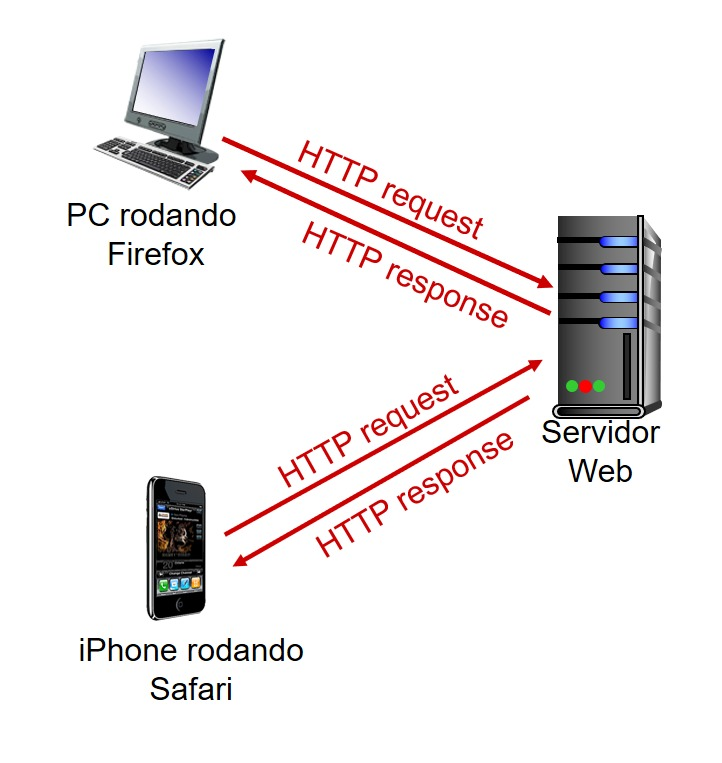
\includegraphics[width=0.5\textwidth]{figuras/reqreshttp}
\begin{flushleft}
\flushleft{Fonte: \citeonline{kurose7th} }
\end{flushleft}
\label{fig:reqreshttp}
}
\end{figure}

Como observado na (Figura~\ref{fig:reqreshttp}), é possível perceber dois clientes se conectando a um único servidor. Cada dispositivo utiliza um navegador diferente em sistemas operacionais e arquiteturas distintas, porém, realizando a requisição HTTP (\textit{request}) e obtendo uma pronta resposta (\textit{response}) do Servidor \textit{Web} em ambas as requisições. O protocolo HTTP funciona independentemente de plataforma, já que, como citado no parágrafo anterior, ele é implementado na camada de Aplicação.

Em cada requisição enviada de um cliente para um servidor, são enviadas também informações detalhadas sobre a requisição, podendo estas irem junto ao corpo (\textit{body}) ou cabeçalho (\textit{header}) da requisição. Podem ser informações sobre o tipo de dado a ser retornado, idioma da resposta ou filtros de dados. Além disso, é passado também um verbo (\textit{HTTP Verb}), que é padrão do protocolo HTTP e define uma série de métodos de requisição responsáveis por indicar a ação a ser executada na representação de um determinado recurso. Cada um deles implementa uma diferente função sendo que alguns recursos são comuns entre todos os verbos. Por exemplo, qualquer método de requisição pode ser do tipo  \textit{safe}, \textit{idempotent}, ou \textit{cacheable}. Abaixo pode-se observar a lista completa de verbos existentes como também seus detalhamentos:
\begin{itemize}
    \item \textbf{GET}~\textemdash~esse método é utilizado para solicitar uma representação de um recurso específico, Requisições utilizando o Método GET devem retornar apenas dados;
    \item \textbf{HEAD}~\textemdash~solicita uma resposta de forma idêntica ao processo que ocorre no tipo GET, porém sem um corpo \textit{body} contendo o recurso;
    \item \textbf{POST}~\textemdash~utilizado para submeter uma entidade a um recurso específico, às vezes causando uma mudança no estado do recurso ou solicitando alterações do lado do servidor;
    \item \textbf{PUT}~\textemdash~substitui todas as atuais representações de seu recurso alvo pela carga de dados da requisição;
    \item \textbf{DELETE}~\textemdash~remove um recurso específico;
    \item \textbf{CONNECT}~\textemdash~estabelece um túnel para conexão com o servidor a partir do recurso alvo;
    \item \textbf{OPTIONS}~\textemdash~usado para descrever as opções de comunicação com o recurso alvo;
    \item \textbf{TRACE}~\textemdash~executa uma chamada de loopback como teste durante o caminho de conexão com o recurso alvo;
    \item \textbf{PATCH}~\textemdash~utilizado para aplicar modificações parciais em um recurso.
\end{itemize}

Atualmente, o protocolo HTTP está passando por uma evolução, saindo da versão 1.1 para o HTTP/2 padronizado no RFC 7540 (\cite{rfc7540}). Em sua mais nova versão, pode-se observar um ganho de performance, visto que ele não é mais um protocolo criado para ser entendido por humanos, mas lido por máquinas. Por esse motivo, é mais eficiente e traz alguns benefícios que consertam os problemas atuais da \textit{Web}. Otimizado, o HTTP/2 usa multiplexação, um nome complicado para dizer que o navegador abre uma única conexão para baixar múltiplos arquivos. Desta forma, as requisições e respostas são paralelas e assíncronas, ou seja, o seu navegador pede vários arquivos ao mesmo tempo e recebe-os assim que eles estiverem prontos, na mesma conexão. Já no HTTP/1.1 (RFC 2616 e versão mais utilizada atualmente) o navegador abre uma conexão para baixar um único arquivo. Se essa conexão ficar ocupada por muito tempo, seja porque o arquivo é muito grande ou porque o servidor está lento para responder, o carregamento da página simplesmente trava no meio do processo. Há como amenizar esse problema abrindo múltiplas conexões, mas isso é apenas uma solução paliativa e, não uma solução permanente. Este trabalho, entretanto, está direcionado a transmitir apenas boas práticas de programação e dicas de otimização de código e performance, evitando soluções paliativas.
%
%
%
\subsection{Navegador}
\label{SubNavegador}

Responsável por toda interação visual do lado cliente (i.e. arquitetura \textit{client-server}), o \textit{browser} ou navegador é quem renderiza as páginas \textit{Web}. Além disso, o navegador trata o DOM (\textit{Document Object Model}), realiza requisições e cuida dos eventos de interação do usuário. Ou seja, sem o navegador, a Internet não teria se desenvolvido tanto quanto vem crescendo nos últimos anos. Isso porque ele deixa tudo mais fácil e intuitivo. Dentre as várias partes de um navegador moderno e funcional, devem ser citado e destacado o motor de renderização, também chamado de mecanismo de renderização, que é quem transforma linguagem de marcação (i.e. HTML, XML, etc.) e informações de formatação (i.e. CSS, XSL, etc.) em um conteúdo formatado para ser exibido em uma tela.

De acordo com o Decálogo da \textit{Web}, definido pelo W3C, qualquer pessoa tem o direito de acessar a informação de forma igualitária. Não importa se o acesso de determinado site é realizado via \textit{tablet}, \textit{desktop}, \textit{smartphone} ou até mesmo a partir de uma TV. Todos têm direito de acessar todas as informações como se estivessem em um \textit{desktop} de última geração. Ainda de acordo com a documentação da W3C, cada um destes meios de acesso utilizam um determinado \textit{browser} para navegar na \textit{Web}.

Todo \textit{browser} carrega apenas um motor de renderização, para o usuário que apenas faz uso do mesmo ao navegar pela \textit{Web}, o processo de faz de forma transparente. No entanto, existem diversos mecanismos de renderização e cada um funciona de maneira distinta para cada dispositivo/equipamento, podendo haver semelhanças ou incompatibilidades entre um e outro. Para o desenvolvedor que é quem constrói um sistema \textit{Web}, não é viável desenvolver um sistema exclusivamente para determinado motor (\textit{engine}). Para tal, a W3C provê uma documentação única e os motores de renderização implementam suas funcionalidades com base nesta documentação a fim de se obter uma padronização ou, no mínimo, um resultado visual eficiente. Portanto, o desenvolvedor precisa apenas utilizar as boas práticas para obter o máximo de produtividade possível e diminuir a quantidade de conflitos por incompatibilidade entre \textit{engines}. Atualmente os dois motores mais utilizados são o \textit{Webkit} e \textit{Gecko} que correspondem aos navegadores: Opera, Safari, Google Chrome, Vivaldi e Brave (\textit{Webkit}, porém, portando para o \textit{Blink}); Mozilla Firefox (\textit{Gecko}, porém, portando para o \textit{Servo}); Além do Internet Explorer (\textit{Spartan}).

Além da renderização o navegador também contém um interpretador JavaScript, também chamado de motor JavaScript, que é um \textit{software} especializado que interpreta e executa JavaScript ou ECMAScript. Assim como os motores de renderização, também existem diversos interpretadores JavaScript. Dentre eles, os mais impactantes são:
\begin{itemize}
    \item \textit{SpiderMonkey}~\textemdash~O primeiro interpretador, criado por Brendan Eich, criador do JavaScript, para o Netscape;
    \item \textit{Squirrelfish Extreme}~\textemdash~Desenvolvido para \textit{Webkit} e desenvolvido pela Google;
    \item \textit{TraceMonkey}~\textemdash~Desenvolvido exclusivamente para o Mozilla Firefox e mais veloz que o concorrente \textit{Webkit};
    \item \textit{V8}~\textemdash~Réplica da Google, uma nova tentativa de se tornar o melhor navegador com o Chrome 2.0. Atual \textit{engine} do navegador.
\end{itemize}

Pode-se observar que há uma disputa por velocidade e otimização entre todos os motores de renderização, interpretadores e afins. Tudo por uma \textit{Web} mais veloz e cada vez mais padronizada (\textit{Web Standards}). A cada dia, novas versões, novos motores e até linguagens surgem para tornar mais veloz a navegação. No momento em que este trabalho foi escrito, destaca-se a existência de implementações do \textit{Web Assembly}, porém, infelizmente, ainda não há versão estável. Portanto, estas implementações não serão citadas neste guia para o desenvolvimento de aplicações \textit{Web}.

\begin{figure}[th]
\centering{
\caption{Árvore DOM.}
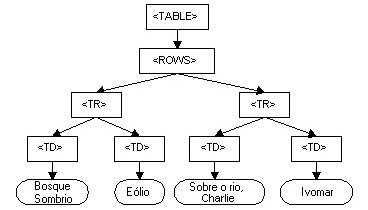
\includegraphics[width=0.5\textwidth]{figuras/domtree}
\begin{flushleft}
\flushleft{Fonte: Retirado de \citeonline{wood2004document} }
\end{flushleft}
\label{fig:domtree}
}
\end{figure}

Não pode-se esquecer do DOM, criado pelo W3C, que é uma multi-plataforma que representa como as marcações em HTML, XHTML e XML são organizadas e lidas pelo navegador. Uma vez indexadas, estas marcações se transformam em elementos de uma árvore que podem ser manipuladas via API. Em outras palavras, pode-se utilizar o DOM para alterar funcionalidades de uma página, tais como o conteúdo, a estrutura ou o estilo.

A (Figura~\ref{fig:domtree}) apresenta a representação gráfica de uma árvore DOM após a leitura de uma tabela HTML. Como percebe-se, o DOM é a base para uma outra árvore que é o que realmente um \textit{browser} monta na tela, a Árvore de Renderização (\textit{Render Tree}). A base para todos os nós da árvore DOM é a classe base chamada \textbf{Node.h}. Ela possui várias categorias, e as relevantes para renderizar código no navegador são os nós de documentos, elementos e texto.
\begin{itemize}
    \item \textbf{Documentos} é o nó mais importante do DOM, com três classes diferentes: \textit{Document}, que é usado por todos os documentos XML e outros que não sejam SVG (que também é um XML, porém com marcação já padronizada), \textit{HTMLDocument} que como o nome diz, cuida de documentos HTML e \textit{SVGDocument}, responsável pelos documentos SVG e também por outros documentos herdados da classe \textit{Document} (Como o \texttt{Document.h} e o \texttt{HTMLDocument.h}).
    \item \textbf{Elementos} são todas as \textit{tags} que estão em arquivos HTML ou XML se transformam em elementos da árvore DOM. Considerando a renderização do navegador, um elemento é um nó com uma \textit{tag} que pode ser usada para fazer subclasses específicas, que podem ser processadas de acordo com as necessidades da árvore de renderização (\texttt{Element.h}).
    \item \textbf{Texto} é propriamente o texto que vai entre os elementos. Todo o conteúdo das \textit{tags}.
\end{itemize}
%
%
%
%
%
%
%
%
%
\section{Tecnologias Básicas de uma Aplicação \textit{Web}}
\label{BaseWeb}

%Quando se estuda sobre Aplicações \textit{Web}, é muito comum se deparar com comparações entre as tecnologias e o mundo real. A mais famosa no contexto de HTML, CSS e JS é:
\begin{quote}
\small{
"HTML é como o pai engenheiro, ele é responsável por estruturar as coisas, garantir que haja um sólido. CSS se parece com a mãe arquiteta, ela embeleza a estrutura, dá brilho e glamour para a criação e fornece o apreço visual pela obra. Já o JS é o filho nerd que brinca com o \textit{Arduino} pela casa, ele faz tudo funcionar, é ele quem faz a mágica acontecer".~Fábio Magnoni.
}
\end{quote}

\subsection{HTML}
\label{SubHTML}

HTML é a sigla em inglês para \textit{HyperText Markup Language}, que, em português significa linguagem para marcação de hipertexto~\footnote{Hipertexto é uma referência aos \textit{links} que interligam páginas, independente se estão localizadas localmente (i.e. mesmo \textit{Website}) ou externamente.}. O HTML é o construtor de blocos mais básico da \textit{Web}. Ela serve para descrever e definir o conteúdo de um documento. Desde a invenção da \textit{Web} por Tim Berners-Lee, a linguagem HTML evoluiu por oito versões, que são: HTML; HTML +; HTML 2.0; HTML 3.0; HTML 3.2; HTML 4.0; HTML 4.01; HTML 5~\footnote{A WHATWG trabalha na versão do HTML5 (observe os espaços), enquanto a W3C se baseia no HTML5 para documentar o HTML 5} (versão atual).

Oficialmente, a W3C, principal organização de padronização da \textit{World Wide Web}, considera apenas 5 versões. Isso deve-se ao fato de duas terem sido criadas antes mesmo da W3C, além do HTML 3.0, nunca lançado oficialmente.

\begin{quote}
\small{
"Tim Berners-Lee acreditava que seria possível interligar hipertextos em computadores diferentes com o uso de links globais, também chamados de hiperlinks. Ele desenvolveu um software próprio e um protocolo para recuperar hipertextos, denominado HTTP. O formato de texto que criou para o HTTP foi chamado de HTML. Tim tomou como base para a criação da HTML a especificação SGML, que é um método internacionalmente reconhecido e aceito, contendo normas gerais para a criação de linguagens de marcação."~\citeonline{html5majour}
}
\end{quote}

Desde sua criação, em 1991, a HTML tem evoluído bastante tanto em sua especificação quanto em seus recursos e escrita. Entretanto, desde o início, ela utiliza marcação (\textit{markup}) para envolver os conteúdos renderizados pelo navegador, tais como textos, imagens e miscelânea. A base do funcionamento está diretamente ligada às \textit{tags} ou etiquetas e também aos atributos. No trecho de Código~\ref{htmlbase}, é importante observar a estrutura básica de um arquivo HTML, chamado de \texttt{index.html}
\begin{lstlisting}[label=htmlbase,caption=Estrutura Básica de um código HTML.]
<!DOCTYPE html>
<html lang="pt-br">
    <head>
        <meta charset="utf-8">
        <title>Monografia</title>
    </head>
    <body>
        <h1>Aqui escrevo minha monografia</h1>
        
        <p>Em <strong>2008</strong> conheci a HTML.</p>
    </body>
</html>
<!-- Salve engano -->

\end{lstlisting}

Após uma breve observação do código, segue abaixo a explicação detalhada de sua estrutura básica:
\begin{itemize}
    \item \textbf{Linha 1}: É declarado o tipo do documento em questão, no caso um arquivo HTML.
    \item \textbf{Linha 2}: É iniciada/aberta a \textit{tag} principal. Logo após, há um atributo chamado \textit{lang} que informa o idioma deste documento HTML.
    \item \textbf{Linhas 3 a 6}: Este é o cabeçalho da página e dentro dele estão contidas informações referentes à página, como codificação e título do documento.
    \item \textbf{Linhas 7 a 11}: Chegamos ao corpo do documento, onde o conteúdo está disponível.
    \item \textbf{Linha 8}: Um elemento de título foi criado e um texto foi inserido dentro deste elemento.
    \item \textbf{Linha 10}: Um elemento de texto \texttt{<p>} é criado, ele é um parágrafo. Seu conteúdo tem um texto simples e um destaque dentro de um elemento \texttt{<strong>} que, por padrão, deixa a fonte em negrito.
    \item \textbf{Linha 12}: Finalização/Fechamento da \textit{tag} principal e fim do código.
    \item \textbf{Linha 13}: Exemplo de comentário.
    \item \textbf{Linha 14}: Apesar de não ser visível, EOF ou Fim do Arquivo, é comum em ambientes UNIX a existência de uma linha em branco em arquivos não vazios. Esta é uma boa prática de desenvolvimento que é adotada neste trabalho.
\end{itemize}

O Resultado do Código~\ref{htmlbase} pode ser observado na Figura~\ref{fig:htmlbase}.

\begin{figure}[th]
\centering{
\caption{Exemplo de Código HTML.}
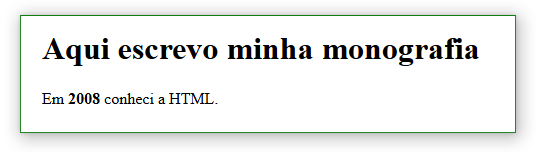
\includegraphics[width=0.5\textwidth]{figuras/htmlbase}
\begin{flushleft}
\flushleft{Fonte: Elaborado pelo autor.}
\end{flushleft}
\label{fig:htmlbase}
}
\end{figure}

É natural delimitar o fechamento de uma \textit{tag} com uma barra~"\texttt{/}"~seguido do restante do nome da \textit{tag} aberta. Elementos desta natureza são chamados de elementos de bloco. Há também os elementos vazios que não necessitam de fechamento de \textit{tag}. No exemplo do Código~\ref{htmlbase}, pode-se perceber a \textit{tag}~\texttt{<meta>}.

Para fins nominais, a terminologia prevê, no exemplo da Linha 10 do Código~\ref{htmlbase}, que há em \texttt{<p>} uma Abertura de \textit{Tag} e em \texttt{</p>} seu fechamento. O que está entre as duas \textit{tags} deste elemento em bloco \texttt{<p>} é o conteúdo, e todo o conjunto se denomina Elemento. Elementos podem conter atributos, que são declarados logo após a abertura da \textit{tag} e separados por um espaçamento. Além disso, os atributos podem ser múltiplos ou inexistentes dentro de um elemento e possuem o padrão de Chave-Valor, onde a chave é declarada inicialmente, seguido por um sinal de igualdade, e o valor é declarado dentro de aspas duplas~\texttt{"valor"}. Ainda na mesma linha 10, observa-se um exemplo de Aninhamento, que é o fenômeno que ocorre quando um elemento é declarado dentro de outro elemento.

A HTML traz para as suas \textit{tags} uma tipografia \textit{case insensitive} (i.e. não diferencia caracteres maiúsculos e minúsculos), ou seja, é possível declarar \texttt{<section>} ou \texttt{<SECTION>} ou até mesmo \texttt{<SeCtIoN>}. No entanto, para garantir um código limpo e fácil de ler e entender por toda a equipe de desenvolvimento, recomenda-se como uma boa prática de desenvolvimento, manter o nome da \textit{tag} em letras minúsculas (ex.: \texttt{<section>}). Adicionalmente, caso um dia seja necessário declarar um elemento com nome composto, a recomendação é utilizar o hífen para separar o nome do elemento, ou seja, declara-se \texttt{MeuElemento} como \texttt{<meu-elemento>}.

É possível aprender HTML de uma maneira muito fácil, pois há diversas fontes de conteúdo na Internet. A fonte mais completa e constantemente atualizada é o diretório HTML em \textit{\citeonline{mdn}}, mantida pela comunidade ativa da Mozilla.
%
%
%
\subsection{CSS}
\label{SubCSS}

CSS (\textit{Cascading Style Sheets}) ou folhas de estilos em cascata é uma linguagem de estilo utilizada para personalizar a apresentação de um documentos \textit{Web}, ou seja, CSS é um padrão de formatação (\textit{Web Standards~\footnote{\textit{Web Standards} é um conjunto de normas, diretrizes, recomendações, notas, artigos, tutoriais e afins de caráter técnico, e destinados a orientar fabricantes, desenvolvedores e projetistas para o uso de práticas que possibilitem a criação de uma \textit{Web} acessível a todos, independentemente dos dispositivos usados ou de suas necessidades especiais.}}) para páginas que permite ir além das limitações impostas pela HTML. Quando se deseja garantir uma formatação homogênea e uniforme em todas as páginas de um site as folhas de estilo em cascata facilitam muito o trabalho de criação.

Quando a HTML foi finalmente implementada, o esforço não foi de maneira alguma, formatar os dados, mas exibir o que previamente foi marcado com as \textit{tags} conhecidas na Subseção~\ref{SubHTML}. Com a popularização da HTML, houve a necessidade de implementar atributos de estilo para alterar algumas aparências da página. Isto fez com que o código ficasse muito complexo e difícil para se manter, visto que tudo estava misturado. Outro fator a se destacar foi a falta de padronização nas implementações dos navegadores daquela época, o que dificultava a visualização das páginas, exibindo conteúdos visualmente distintos entre \textit{browsers}. Estes problemas infelizmente ainda acontecem, porém, pode ser minimizado com boas práticas, como separar o código HTML do CSS e utilizar abordagens mais genéricas e/ou bibliotecas CSS previamente testadas pela comunidade ativa de desenvolvedores. Isso permite evitar o retrabalho por parte do programador, pois o mesmo pode utilizar ferramentas existentes e focar apenas no produto, realizando apenas pequenas intervenções. Tudo isso permite a garantia de uma melhor experiência \textit{cross-browser}~\footnote{\textit{Cross-Browser} refere-se à habilidade de um site suportar múltiplos navegadores sem comprometer o estilo previamente implementado.} e \textit{cross-platform}~\footnote{\textit{Cross-Platform} é a denominação de uma Aplicação \textit{Web} que foi desenvolvida para funcionar independente de plataforma.} para o usuário.

Em 1994, Håkon Wium Lie e Bert Bos propuseram a criação do CSS, após observarem todo este cenário caótico no desenvolvimento de Aplicações \textit{Web}, uma maneira mais fácil de formatar a apresentação da página. Em 1995 a proposta foi apresentada ao \textit{World Wide Web Consortium} (W3C), o qual é uma comissão que define os padrões de programação para a WWW. Recém criada, a W3C demonstrou interesse pelo projeto e montou uma equipe de desenvolvimento que viria a finalizar seu primeiro projeto em 1996. Foi assim que surgiu a primeira versão do CSS. A história do CSS é descrita em mais detalhes no capítulo 20 do livro CSS: Projetando para a \textit{Web}, escrito pelos próprios criadores \citeonline{lie2005cascading}.

Atualmente, o CSS encontra-se em sua versão estável de número 3 (CSS 3) e em desenvolvimento da versão 4 (CSS 4), proposta por~\citeonline{css4}~nos diretórios da W3C. As evoluções do CSS trouxeram mais recursos e aumentaram a sua abrangência, porém, mantendo o mesmo princípio de formatar a aparência das páginas \textit{Web}. Inicialmente, apenas cores eram mudadas. Após isso, o comportamento pode ser manipulado também. Então foi possível definir o tamanho dos elementos apenas com CSS e por fim, temos animações e efeitos em 3D, além de cada vez mais suporte à responsividade~\footnote{Design Responsivo é uma técnica de estruturação HTML e CSS, em que o site se adapta ao browser do usuário sem precisar definir diversas folhas de estilos para cada resolução.}.

É possível inserir regras de estilo em cascata de três formas junto a um documento HTML. São elas:
\begin{itemize}
    \item \textit{Inline}~\textemdash~via atributo HTML, adicionando ao atributo \texttt{style} o seu código CSS. Desta forma, o código inserido refletirá sobre o elemento ao qual a propriedade foi declarada.
    \item \textit{Embedding}~\textemdash~via \textit{tag} \texttt{<style>}. Dentro do cabeçalho (\texttt{<head>}), é possível inserir trechos genéricos de código CSS. Podendo aplicá-los a todo o documento ou apenas a trechos específicos.
    \item \textit{Linking}~\textemdash~utilizando um ou mais arquivos externos de folha de estilo em cascata com a extensão \texttt{.css}, importados dentro do documento HTML.
\end{itemize}

O \textit{Linking} é considerado a melhor prática para se trabalhar com folhas de estilo em cascata, pois, além de ser a maneira mais recomendada, é também a estratégia mais organizada para descentralizar o estilo \textit{inline} dos componentes. Em outras palavras, utilizando o atributo \texttt{<style>}. A vantagem de se utilizar uma importação \textit{Linking} ao invés de \textit{Embedding} se resume pelo fato de reduzir o tamanho de linhas no documento HTML, garantindo uma melhor leitura de código e separação das tecnologias, com o objetivo de facilitar a manutenção de código.

A estrutura de código CSS, assim como HTML é muito fácil de aprender. Juntamente ao arquivo \texttt{index.html} (Código~\ref{htmlbase}), cria-se um outro arquivo chamado \texttt{style.css}, que contém o código CSS (Código~\ref{cssbase}). As regras de estilização podem ser observadas logo abaixo.
\begin{lstlisting}[label=cssbase,caption=Exemplo de um código CSS.]
/* h1 vai ser vermelho */
h1 {
    color: red;
}

/* o paragrafo tera uma borda azul */
p {
    border: 1px solid blue;
}
\end{lstlisting}

Como descrito através dos comentários do código acima, observam-se duas modificações visuais. A primeira é a cor vermelha no elemento de título~"\texttt{<h1>}"~e a segunda está relacionada ao parágrafo com a definição de uma borda na cor azul. Diferente do atributo de cor~"\texttt{color}"~que tem apenas uma propriedade, o atributo de borda~"\texttt{border}"~possui três propriedades, que são: 
\begin{itemize}
    \item \textbf{Tamanho}~\textemdash~O tamanho foi definido em \textit{pixels}, mas existem diversas outras unidades de medida disponíveis no CSS como \texttt{px}, \texttt{rem}, \texttt{rm}, \texttt{em}, \texttt{ch}, \texttt{\%} dentre outras.
    \item \textbf{Estilo}~\textemdash~O tipo da borda escolhido foi a simples. Ou seja, uma borda sólida com a espessura previamente definida através do tamanho. Além disso, poderia ser uma borda pontilhada~"\texttt{dashed}", dupla~"\texttt{double}"~ou outro tipo de borda.
    \item \textbf{Cor}~\textemdash~A cor pode ser definida pelo nome em inglês ou por meio de uma codificação em RGB~"\texttt{rgb(0, 0, 255)}"~ou hexadecimal~"\texttt{\#0000ff}", por exemplo.
\end{itemize}

Todos estes detalhes e valores das propriedades CSS podem ser consultadas no \textit{\citeonline{mdn}} do diretório CSS. 

É importante destacar a estrutura do bloco, inicialmente um seletor é declarado e logo após chaves "\texttt{{ }}" são abertas e o código é inserido dentro delas. É possível perceber a semelhança com os atributos HTML pelo fato de existir um sistema de chave e valor, separados pelos dois pontos "\texttt{:}" e finalizando o comando com ponto e vírgula "\texttt{;}". Apesar deste ser um guia de boas práticas, não são utilizadas classes no código de exemplo. Para utilizar classes na HTML basta atribuir \texttt{class="titulo"} no elemento \texttt{<h1>} e, em seguida, alterar a linha 2 para \texttt{.titulo} no código CSS. O ponto é um identificador de classe~\footnote{O identificador ponto~"\texttt{.}"~a frente do nome do seletor indica uma classe e o identificador cerquilha~"\texttt{\#}"~referencia um identificador único (i.e. \texttt{id="titulo"}).}.

Para garantir o pleno funcionamento e ligar o código de estilo ao arquivo \texttt{index.html}, é necessário importá-lo. Para isso, basta adicionar dentro do cabeçalho do Código~\ref{htmlbase} o trecho de código disponível em~\ref{inserircssnohtml}, que é um elemento de \textit{link}. Desta forma, seus atributos \texttt{rel} e \texttt{type} definem uma folha de estilo do tipo CSS e o atributo \texttt{href} informa o caminho onde está localizado o arquivo \texttt{style.css} em questão. Neste exemplo, o arquivo localiza-se no mesmo diretório do arquivo \texttt{index.html} criado.
\begin{lstlisting}[label=inserircssnohtml,caption=Inserir CSS externo no HTML.]
<link rel="stylesheet" type="text/css" href="style.css" />
\end{lstlisting}

Como resultado das implementações, é possível observar na Figura~\ref{fig:cssbase}, uma página \textit{Web} mais colorida.

\begin{figure}[th]
\centering{
\caption{Exemplo de Código CSS.}
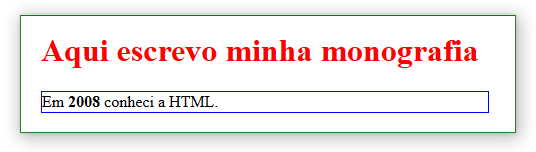
\includegraphics[width=0.5\textwidth]{figuras/cssbase}
\begin{flushleft}
\flushleft{Fonte: Elaborado pelo autor.}
\end{flushleft}
\label{fig:cssbase}
}
\end{figure}

É importante salientar que as boas práticas existem para evitar erros e confusões no desenvolvimento do projeto. Se tratando de CSS, um dos maiores problemas está relacionado à precedência. Em outras palavras, é necessário evitar que duas regras de estilo sejam aplicadas para um mesmo elemento HTML especificado. Por exemplo, se houver diferentes modos de estilo (exemplo: \textit{Inline} e \textit{Linking}) as especificações podem entrar em conflito. Desta forma, o navegador é responsável por intermediar e decidir qual estilo conflitante deverá prevalecer baseado em quem tem maior ordem de precedência. A ordem de precedência adotada pelos navegadores felizmente é padronizada e sua definição é:
\begin{itemize}
    \item \textit{Inline} ou Estilo em linha~\textemdash~dentro de um elemento HTML.
    \item \textit{Embedding} ou Folha de estilo incorporada~\textemdash~definida no cabeçalho do documento.
    \item \textit{Linking} ou Folha de estilo externa~\textemdash~importada e referenciada.
    \item \textit{Default} ou Estilo padrão do navegador~\textemdash~estilo predefinido.
\end{itemize}

É importante lembrar esta ordem de precedência para que se saiba qual valor de estilo tem maior prioridade. Assim sendo, um estilo \textit{inline} tem a prioridade mais elevada, o que significa que prevalece sobre aquele definido no cabeçalho do documento, que, por sua vez, é prioritário em relação ao definido em uma folha de estilo em cascata externa e esse sobre o formato que o navegador especifica~\footnote{É comum utilizar estilos CSS para reiniciar a aparência padrão do navegador, visto que, os navegadores apresentam pré-formatações de estilo distintas. Esta é uma boa prática.}.

Para os estilos \textit{Embedding} e \textit{Linking} onde o código é definido por blocos, há a possibilidade de se tratar a herança além de pseudo-classes~\footnote{Uma pseudo-classe CSS é uma palavra-chave adicionada aos seletores que especifica um estado especial do elemento a ser selecionado.}. Por exemplo, quando o usuário passa o ponteiro do mouse sobre determinado elemento, este evento ou estado especial é chamado de \textit{hover} e pode ser inserido \texttt{:hover} após o seletor CSS (exemplo: \texttt{h1:hover \{}). Isto faz com que o evento de \textit{hover} seja acionado e um estilo, normalmente diferente do inicialmente renderizado, seja aplicado ao elemento que ativou o evento em questão. Existem diversas pseudo-classes que identificam diversos eventos de página, tanto em relação aos eventos causados pela interação do usuário com a aplicação (exemplo: \texttt{:hover}) quanto eventos de estado de elementos (exemplo: \texttt{:disabled}) e até herança (exemplo: \texttt{:first-child}). Portanto, as pseudo-classes para seletores CSS, tem tornado o desenvolvimento muito mais fácil e intuitivo.

\begin{figure}[th]
\centering{
\caption{Modelo de Caixa no CSS.}
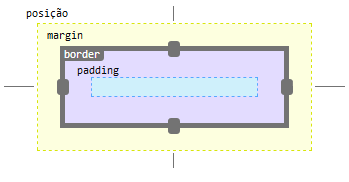
\includegraphics[width=0.5\textwidth]{figuras/boxmodel}
\begin{flushleft}
\flushleft{Fonte: Developer Tools do Mozilla Firefox Nightly (61.0a1).}
\end{flushleft}
\label{fig:boxmodel}
}
\end{figure}

Outros detalhes importantes sobre CSS estão relacionados à orientação das margens (\textit{margin}), preenchimentos (\textit{padding}) e bordas (\textit{border}). Na Figura~\ref{fig:boxmodel}, é possível observar cada uma das orientações. O espaçamento externo ao elemento definido por~\texttt{margin}~e interno definido por~\texttt{padding}, que distancia o conteúdo do elemento das bordas, que, trivialmente é definido por por~\texttt{border}.
%
%
%
\subsection{JavaScript}
\label{SubJS}

JavaScript, ou simplesmente JS, é uma linguagem de programação de alto nível, dinâmica e interpretada do lado cliente (i.e. processada pelo navegador), desenvolvida por Brendan Eich. O JavaScript, juntamente com HTML e CSS é um dos três pilares que atualmente sustentam a rede mundial de computadores (\textit{World Wide Web}). No entanto, o JS é o principal responsável por tornar as páginas da \textit{Web} interativas. Foi originalmente desenvolvido com o nome de Mocha. Posteriormente, teve seu nome modificado para LiveScript e, por fim, JavaScript. LiveScript foi o nome oficial da linguagem quando ela foi lançada pela primeira vez, na versão beta do navegador Netscape 2.0, em setembro de 1995. Entretanto, teve seu nome alterado em um anúncio conjunto com a \textit{Sun Microsystems}, em dezembro do mesmo ano, quando foi implementado no navegador Netscape, versão 2.0B3.

Neste instante, a Netscape percebeu que a WWW precisava se tornar mais dinâmica, com o objetivo de realizar tarefas simples como verificar se os usuários inseriam valores corretos em um formulário. Algo dessa natureza precisaria enviar os dados para um servidor, para que esse interpretasse os dados e retornasse uma saída.

A linguagem é padronizada pela~\citeonline{ecma}, uma associação Europeia para a padronização de comunicação e informação. Esta versão padronizada de JavaScript, chamada ECMAScript, comporta-se da mesma forma em todas as aplicações que suportam o padrão. Ou seja, as empresas podem usar a linguagem de padrão aberto para desenvolver a sua implementação de JavaScript. O padrão ECMAScript é documentado na especificação ECMA-262 e encontra-se disponível em~\citeonline{specification1999standard}.

Com o JavaScript é possível criar efeitos especiais para nossas páginas na \textit{Web}, além da possibilidade de explorar uma maior interatividade com nossos usuários. Além disso, o JavaScript é uma linguagem orientada a objetos, ou seja, ela trata todos os elementos da página como objetos distintos, facilitando a tarefa da programação também em multiplataforma.

A sintaxe da linguagem é bastante similar à linguagem C. Apesar de usar Java no nome, as duas linguagens são distintas. Outra curiosidade sobre o JavaScript, é que a linguagem apresenta recursos não disponíveis em C, C++ e em Java, já que ela teve fortes influências das linguagens de script, tais como Awk, Perl e Python. Os \textit{scripts} desenvolvidos em JavaScript são muito populares e amplamente integrados em páginas \textit{Web} devido à facilidade de interação com o \textit{Document Object Model} (DOM). Atualmente, JavaScript é a principal linguagem para programação client-side em navegadores \textit{Web}. Foi concebida para ser uma linguagem script com orientação a objetos baseada em protótipos, tipagem fraca e dinâmica e funções de primeira classe. Possui suporte à programação funcional e apresenta recursos como fechamentos e funções de alta ordem comumente indisponíveis em linguagens populares como Java e C++. É também a linguagem de programação mais utilizada do mundo por ser a única existente para realizar as interações nos navegadores, o que explica facilmente sua fácil difusão. São características da linguagem:
\begin{itemize}
    \item \textbf{Imperativa e Estruturada}~\textemdash~Suporta os elementos de sintaxe comuns em programação estruturada (exemplo: \texttt{if}, \texttt{while}, \texttt{switch}), com a exceção do escopo. Nativamente, o escopo em JavaScript é definido com base no nível de função, porém há suporte para escopo a nível de bloco através do comando \texttt{let}. Diferente da linguagem C, o JavaScript traz o uso do ponto-e-vírgula como opcional ao fim dos comandos. No entanto, é uma boa prática utilizá-lo.
    \item \textbf{Dinâmica}~\textemdash~Assim como na maioria das linguagens de \textit{script}, a tipagem é dinâmica, não associando o tipo a variável, mas ao valor~\footnote{Em programação de computadores com linguagens de programação orientadas a objetos, \textit{duck typing} é um estilo de tipagem em que os métodos e propriedades de um objeto determinam a semântica válida, em vez de sua herança de uma classe particular ou implementação de uma interface explicita.}, o que garante uma grande tolerância a erros, uma vez que as conversões automáticas são realizadas durante operações. JavaScript é quase inteiramente baseada em objetos, sendo estes, \textit{arrays} associativos, aumentados com protótipos. Em tempo de execução, as propriedades e seus valores podem ser adicionadas, mudadas, ou deletadas. Além disso, através do comando \textit{eval}, é possível executar comandos da linguagem que estejam escritos em uma \textit{string}. Um exemplo tradicional é quando uma variável possui um determinado valor inteiro em momento e um valor textual em outro instante.
    \item \textbf{Funcional}~\textemdash~As funções são de primeira classe. Isto é, são objetos que possuem propriedades e métodos, que podem ser passados como argumentos, serem atribuídos às variáveis ou retornados como qualquer outro objeto. Há suporte também para funções aninhadas~\footnote{Funções 'internas' ou 'aninhadas' são funções definidas dentro de outras funções. São criadas cada vez que a função que as contém (externa) é invocada. Além disso, o escopo da função externa, incluindo constantes, variáveis locais e valores de argumento, se transforma parte do estado interno de cada objeto criado a partir da função interna, mesmo depois que a execução da função interna é concluída.} e fechamentos~\footnote{JavaScript permite que funções aninhadas sejam criadas com o escopo léxico no momento de sua definição e possui o operador () para invocá-las em outro momento. Essa combinação de código que pode ser executado fora do escopo no qual foi definido, com seu próprio escopo durante a execução.}.
    \item \textbf{Baseada em Protótipos}~\textemdash~Para seu mecanismo de herança, a linguagem utiliza protótipos ao invés de classes. É possível simular diversas características de orientação a objetos (OO) baseada em classes com protótipos. Ou seja, não há distinção entre a definição de função e método. A distinção ocorre durante a chamada da função; função pode ser chamada como um método, neste caso, a \textit{keyword} \texttt{this} é associada àquele objeto via tal invocação.
\end{itemize}

A segurança da linguagem é um ponto importante a discutir. A junção do JavaScript e DOM representam uma potencialidade para programadores maliciosos escreverem \textit{scripts} para rodarem em clientes \textit{Web}. Os navegadores são projetados para mitigar riscos. Por exemplo, o JavaScript utiliza uma \textit{sandbox}~\footnote{O conceito do \textit{Sandbox} é bem semelhante ao de criar uma máquina virtual, de fato, esse método é considerado um tipo de virtualização. Porém, esse sistema é muito mais focado em segurança.}, onde apenas ações relacionadas à Internet podem ser executadas, não tarefas de proposito geral. Isso impede que o escopo de código acesse informações do Sistema Operacional (SO), bem como dos dados do usuário (exemplo: credenciais, arquivos). A maioria dos \textit{bugs} em JavaScript relacionados à segurança são brechas de uma das regras implementadas em determinado cliente \textit{Web}.

JavaScript  tem uma biblioteca padrão de objetos, como: \texttt{Array}, \texttt{Date}, e \texttt{Math}, e um conjunto de elementos que formam o núcleo da linguagem, tais como: operadores, estruturas de controle e declarações. O núcleo do JavaScript pode ser estendido para uma variedade de propósitos, complementando assim a linguagem:~\textit{O lado cliente do JavaScript}~\textemdash~estende-se do núcleo da linguagem, fornecendo objetos para controlar um navegador \textit{Web} e seu DOM. Por exemplo, as extensões do lado do cliente permitem que uma aplicação coloque elementos em um formulário HTML e responda a eventos do usuário, como cliques do mouse, entrada de formulário e de navegação da página. \textit{O lado do servidor do JavaScript}~\textemdash~fornece objetos relevantes à execução do JavaScript em um servidor. Por exemplo, as extensões do lado do servidor permitem que uma aplicação comunique-se com um banco de dados, garantindo a continuidade de informações de uma chamada para a outra da aplicação, ou executar manipulações de arquivos em um servidor.

Há diversas expressões e operadores disponíveis na linguagem: Expressões primárias e \textit{left-hand-side}; Incremento e decremento; Operadores unários, aritméticos, relacionais, de igualdade, de deslocamento bit a bit, lógicos binários, bit a bit binários, ternários e de atribuição, além do operador vírgula.

A sintaxe básica, como citada anteriormente, é produto da união de várias linguagens, incorporando recursos e estruturas. JavaScript é \textit{case-sensitive}~\footnote{\textit{Case-sensitive} é um anglicismo que se refere a um tipo de análise tipográfica da informática onde há diferenciação entre maiúsculas e minúsculas.} e utiliza um conjunto de caracteres Unicode~\footnote{Unicode é um padrão que permite aos computadores representar e manipular, de forma consistente, texto de qualquer sistema de escrita existente.}. No bloco de Código~\ref{jsbase}, pode ser visualizado um exemplo de operações básicas da linguagem. Atente ao fato das linhas 1 e de 4 a 6 representarem comentários, em linha e em múltiplas linhas, respectivamente. Além das declarações de variáveis nas linhas 2 e 7 utilizarem o operador~\texttt{var}, sendo que existem também os operadores~\texttt{let}~e~\texttt{const}, usados para declarar variáveis locais em escopo de bloco e constantes de apenas leitura. Ainda na linha 7, a \textit{string} foi revestida com aspas duplas para representar o tipo \textit{string}. Além deste caractere, as aspas simples ou crases também podem ser utilizadas para delimitar o conteúdo. A linha 9 traz uma declaração de função sem parâmetros de entrada, os parâmetros poderiam ser declarados entre os parênteses "\texttt{()}". Por fim, na linha 13 a função~\texttt{exibirDados()}, previamente declarada é invocada, como resultado esperado teremos~\texttt{"Aracati, 2018"}. Os resultados podem ser visualizados no console do navegador, haja visto que foi utilizado a função nativa~\texttt{console.log()}~que imprime um log no console do cliente onde o \textit{script} é executado.

\begin{lstlisting}[label=jsbase,caption=Exemplo de um código JS.]
// Declarar ano
var ano = 2018;

/* Declarar
   cidade
*/
var cidade = "Aracati";

function exibirDados() {
    console.log(cidade, ano);
}

exibirDados();
\end{lstlisting}

O rascunho mais recente da ECMA-262 atualmente é o~\citeonline{ecma2019}~para 2019. Porém como no presente momento encontra-se em estado de \textit{draft}, o padrão ECMA-262 \textit{Edition} 6 (ES6) ou como é oficialmente chamado, ECMAScript 2015, é a versão mais sólida e por esta razão foi escolhida como referência para este trabalho. O ES6 define sete tipos de dados para a linguagem JavaScript, os objetos "\texttt{Object}" e outros seis tipos que são:
\begin{itemize}
    \item \textit{Number}~\textemdash~Números inteiros ou de ponto flutuante.
    \item \textit{String}~\textemdash~Cadeia de caracteres.
    \item \textit{Boolean}~\textemdash~Valor binário entre~\texttt{true}~e~\texttt{false}.
    \item \textit{Symbol}~\textemdash~Tipo de dado com instâncias únicas e imutáveis.
    \item \textit{undefined}~\textemdash~Propriedade de valor indefinido.
    \item \textit{null}~\textemdash~Indicação de Valor nulo, existente, porém nulo.
\end{itemize}

A condição de existência é muito básica, em testes condicionais a linguagem entende~\texttt{false},~\texttt{null},~\texttt{undefined}, zero~"\texttt{0}"~e \textit{string} vazia~"\texttt{""}"~como negações e qualquer valor distinto como afirmação (i.e.~\texttt{true}). Tal comparação pode ser reproduzida com o operador lógico NOT~"\texttt{!}"~que retorna falso caso o único operando possa ser convertido para verdadeiro; senão, retorna verdadeiro. Com isto, é possível executar um teste de existência utilizando o NOT duas vezes~\footnote{Este é um artificio pouco conhecido, entretanto, sua utilização é bastante fácil e útil para testar muitos casos lógicos com~\texttt{!!}, funciona como um conversor booleano nativo da linguagem. Assim como utilizar~\texttt{+}, converte para numérico.}.

A precedência de operadores determina a ordem em que eles são aplicados quando uma expressão é avaliada. Assim como na álgebra, o usuário pode substituir a precedência dos operadores utilizando parênteses. É possível observar a descrição da precedência de operadores (Tabela~\ref{tab:jsPrecedenciaOperadores}) em ordem decrescente.

\begin{table}[th]
\centering
\caption{Operadores de Precedência.}
\label{tab:jsPrecedenciaOperadores}
\begin{tabular}{llll}
Tipo de operador                &   Operadores individuais\\\hline
membro                          &   \texttt{. []}\\
chamada / criação de instância  &   \texttt{() new}\\
negação / incremento            &   \texttt{!~\textasciitilde~$-$~$+$~$++$~$--$~typeof void delete}\\
multiplicação / divisão         &   \texttt{* / \%}\\
adição / subtração              &   \texttt{+ -}\\
deslocamento bit a bit          &   \texttt{$<<$~$>>$~$>>>$}\\
relacional                      &   \texttt{< <= > >= in instanceof}\\
igualdade                       &   \texttt{== != === !==}\\
E bit a bit                     &   \texttt{\&}\\
OU exclusivo bit a bit          &   \texttt{\^}\\
OU bit a bit                    &   \texttt{|}\\
E lógico                        &   \texttt{\&\&}\\
OU lógico                       &   \texttt{||}\\
condicional                     &   \texttt{?:}\\
atribuição                      &   \texttt{= += -= *= /= \%=~$<<$=~$>>$=~$>>>$=~\&=~$\hat{}$= |=}\\
vírgula                         &   \texttt{,}\\
\hline
\end{tabular}
\begin{flushleft}
\flushleft{Fonte: Operadores de Precedência em~\textit{\citeonline{jsoperatorprecedence}}.}
\end{flushleft}
\end{table}

Assim como nas subseções anteriores e pertencentes a Seção~\ref{BaseWeb}, esta subseção também utiliza o trecho de código HTML como base (Código~\ref{htmlbase}), acrescentando as formações de estilo citadas ao longo da Subseção~\ref{SubCSS}, bem como suas referências de arquivos criados (\texttt{index.html}~e~\texttt{style.css}) para fins de exemplo contínuo ao longo da seção. Como produto das modificações citadas anteriormente, pode-se observar a estrutura final HTML no trecho de Código~\ref{htmlfinal}. Além disso, há a necessidade de criar um novo arquivo chamado~\texttt{app.js}~para a inserção do código JavaScript que é responsável pela interação da página.
\begin{lstlisting}[label=htmlfinal,caption=Documento HTML com CSS e JS.]
<!DOCTYPE html>
<html lang="pt-br">
    <head>
        <meta charset="utf-8">
        <title>Monografia</title>
        <link rel="stylesheet" href="style.css">
    </head>
    <body>
        <p>Oi <strong class="name"></strong> tudo bem?</p>
        <button onclick="rename(this)">Ronaldo</button>
        
        <script src="app.js"></script>
    </body>
</html>
\end{lstlisting}

Neste ponto, observa-se um documento HTML modificado, com ligações para um arquivo de estilo CSS e um arquivo de \textit{script} JS. Este \textit{script} ainda inexistente, é descrito no bloco de Código~\ref{appjs}, logo abaixo. Este arquivo objetiva prover uma interação na página, modificando-a através do DOM.

\begin{lstlisting}[label=appjs,caption=Exemplo de um código JS.]
function rename(el) {
    const strong = document.querySelector('.name');
    strong.innerText = el.innerText;
}
\end{lstlisting}

O resultado pode ser observado nas figuras~\ref{fig:jsbase}~e~\ref{fig:htmlfinal}, onde a página mantém o mesmo arquivo~\texttt{style.css}, imutável, adicionado um botão com um evento de \textit{click} que altera parte do texto do elemento \texttt{<p>} de nosso HTML.

\begin{figure}[th]
\centering{
\caption{Exemplo de Código JS.}
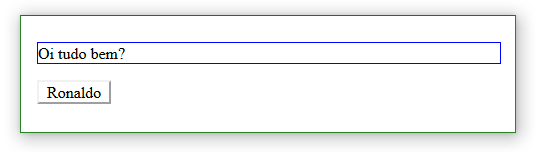
\includegraphics[width=0.5\textwidth]{figuras/jsbase}
\begin{flushleft}
\flushleft{Fonte: Elaborado pelo autor.}
\end{flushleft}
\label{fig:jsbase}
}
\end{figure}

No arquivo~\texttt{app.js}, uma função chamada~\texttt{rename()}~recebe como parâmetro (\texttt{el}) o elemento que a invoca através do evento de~\texttt{onclick=}~do botão. Após isto, o elemento que contém a classe~\texttt{.name} é renomeado para o mesmo texto de dentro do botão (i.e. Ronaldo). Como observado no na linha 9 do Código~\ref{htmlfinal}, dentro do elemento parágrafo~"\texttt{<p>}"~há um texto livre e dentro deste, um elemento~\texttt{<strong>}~com a classe~\texttt{.name}~que receberá o texto do botão. Na Figura~\ref{fig:htmlfinal}~é possível observar o resultado desta interação. É importante ressaltar que o texto recém adicionado como retorno do evento está em negrito por formatação padrão do elemento~\texttt{<strong>}~no navegador em questão e que esta aparência inicial pode ser personalizada com uma folha de estilo.

\begin{figure}[th]
\centering{
\caption{Documento HTML com CSS e JS.}
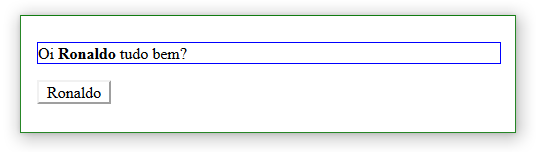
\includegraphics[width=0.5\textwidth]{figuras/htmlfinal}
\begin{flushleft}
\flushleft{Fonte: Elaborado pelo autor.}
\end{flushleft}
\label{fig:htmlfinal}
}
\end{figure}

Além do exemplo apresentado, onde foi realizada uma interação simples na página. É possível com a linguagem JavaScript: Criar validações em formulário, realizar troca de dados com o servidor, computar dados e até gerenciar recursos. Nesta subseção apenas exemplos de JavaScript para \textit{Front-End} foram apresentados, porém, é possível executá-lo no \textit{Back-End}, bem como, Banco de Dados e Sistemas Operacionais também podem ser criados com a linguagem. O grande diferencial da linguagem, além da exclusividade na \textit{Web}, é a comunidade participativa muito responsável pela grande difusão e manutenção de novas soluções com a linguagem.
%
%
%
%
%
%
%
%
%
\section{Elementos Básicos para uma Aplicação \textit{Web} Moderna}
\label{ElementosWeb}

\subsection{AJAX}
\label{SubAJAX}

AJAX significa \textit{Asynchronous JavaScript and XML}, uma técnica para criar aplicações \textit{Web} melhores, mais rápidas e interativas com a ajuda de XML, HTML, CSS e JavaScript. Foi apresentado ao mundo em~\citeonline{garrett2005ajax}, descrevendo a técnica onde dados podem ser carregados em segundo plano sem necessidade de recarga de página. Isso resultou no ressurgimento do JavaScript, sustentado por novas comunidades, bibliotecas e \textit{frameworks}.

Em aplicações \textit{Web} convencionais, o \textit{front-end} transmite informações para o \textit{back-end} utilizando solicitações síncronas. Isso significa, por exemplo, que um formulário é preenchido, o botão de enviar é acionado e há um redirecionamento para uma nova página com novas informações retornadas do servidor. Com o AJAX, quando o formulário é submetido ao servidor, diferentemente do modo síncrono padrão, o JavaScript realiza uma solicitação ao servidor, interpreta os resultados e atualiza a tela atual. No sentido mais puro, o usuário nunca sabe que algo foi transmitido ao servidor.

AJAX é uma tecnologia \textit{Web} independente de software e de servidor, baseada em \textit{Open Standards} (i.e. Padrões Abertos). É comum o uso de XML como formato para o recebimento de dados do servidor, embora qualquer formato, incluindo texto simples, possa ser usado. Utiliza o paradigma \textit{data-driven} em vez de \textit{page-driven}, o que permite que o usuário continue utilizando a aplicação enquanto o AJAX solicita informações do servidor, tudo em segundo plano e assíncrono através de objetos de requisição~\texttt{XMLHttpRequest}, próprios do navegador. AJAX é capaz de realizar requisições em todos os verbos HTTP disponíveis na Subseção~\ref{SubHTTP}~e utiliza JavaScript para fazer tudo.
%
%
%
\subsection{JSON}
\label{SubJSON}

JSON é o acrônimo de \textit{Javascript Object Notation} ou Objeto de Notação JavaScript. É um formato leve de intercâmbio de dados padronizado no RFC 4627 em \citeonline{crockfordrfc}. Para seres humanos, é fácil de ler e escrever, para máquinas, é fácil de interpretar e gerar. Está baseado em um subconjunto da linguagem JavaScript, a notação, origem do nome. JSON é bastante similar ao XML, com a mesma utilidade, mesmo intuito, porém mais leve. Apesar do nome ser bem sugestivo, não necessariamente deve ser utilizado com JavaScript, é um formato de texto e completamente independente de linguagem. Muitas linguagens hoje em dia dão suporte ao JSON, é meio que um novo método, substituto do antigo e conhecido XML. Ele é muito usado para retornar dados vindos de um servidor utilizando requisições AJAX para atualizar dados em tempo real. JSON está constituído em duas estruturas:
\begin{itemize}
    \item Uma coleção de pares nome/valor. Em várias linguagens, isto é caracterizado como um \textit{object}, dicionário, \textit{hash table} ou arrays associativas.
    \item Uma lista ordenada de valores. Na maioria das linguagens, isto é caracterizado como uma \textit{array}, vetor, lista ou sequência.
\end{itemize}

Estas são estruturas de dados universais. Em JSON, os dados são apresentados desta forma: Um objeto é um conjunto desordenado de pares nome/valor. Um objeto começa com uma chave de abertura~"\texttt{\{}"~e termina com uma chave de fechamento~"\texttt{\}}". Cada nome é seguido por dois pontos~"\texttt{:}"~e os pares nome/valor são seguidos por vírgula~"\texttt{,}". Uma \textit{array} é uma coleção de valores ordenados. O \textit{array} começa com colchete de abertura~"\texttt{[}"~e termina com colchete de fechamento~"\texttt{]}". Os valores são separados por vírgula. Por final, um valor pode ser uma cadeia de caracteres, um número, booleano, valor nulo, objeto ou até uma \textit{array}. As estruturas podem estar aninhadas.

\begin{lstlisting}[label=basejson,caption=Exemplo de um arquivo JSON.]
{
  "letras" : [
    { "letra": "A", "numeros": [ { "numero": 5 }, { "numero": 10 } ] },
    { "letra": "B", "numeros": [ { "numero": 7 }, { "numero": 17 } ] },
    { "letra": "C", "numeros": [ { "numero": 9 }, { "numero": 33 } ] }
  ]
}
\end{lstlisting}

Nos códigos~\ref{basexml}~e~\ref{basejson}, é possível observar o quão menor é o arquivo JSON em comparação ao XML, visto que sua estrutura contribui por ser um formato de texto mais simplificado. Os blocos de código contêm, respectivamente para XML e JSON, 509 e 237 caracteres. Uma diminuição de aproximadamente 53\% na quantidade de caracteres necessária para se chegar ao mesmo resultado. Optar pela utilização do JSON em relação ao XML é uma forma de otimização, visto a menor quantidade de dados a serem processados e posteriormente trafegados em rede.

\begin{lstlisting}[label=basexml,caption=Exemplo de um arquivo JSON.]
<?xml version="1.0" encoding="UTF-8"?>
<root>
    <letras>
        <letra>A</letra>
        <numeros>
            <numero>5</numero>
            <numero>10</numero>
        </numeros>
    </letras>
    <letras>
        <letra>B</letra>
        <numeros>
            <numero>7</numero>
            <numero>17</numero>
        </numeros>
    </letras>
    <letras>
        <letra>C</letra>
        <numeros>
            <numero>9</numero>
            <numero>99</numero>
        </numeros>
    </letras>
</root>
\end{lstlisting}
%
%
%
%
%
%
%
%
%
\section{Arquitetura de uma Aplicação}
\label{ArquiteturaWeb}

\subsection{MVC \textit{versus} VMP \textit{versus} MVVM}
\label{SubMVCMVVM}

O principal ponto de partida para decidir qual padrão arquitetural a escolher, é entender suas particularidades e semelhanças, comparando quais as melhores descrições em uma abordagem para o desenvolvimento de software.

Os padrões apresentam objetivos semelhantes, contudo o fazem de maneira distinta e estes objetivos almejam aumentar a modularidade, flexibilidade, testabilidade e manutenibilidade do código. Ainda sobre as semelhanças nas responsabilidades dentro da aplicação, devemos descrevê-las como:
\begin{itemize}
    \item \textit{Model}~\textemdash~Responsável pelo acesso aos dados, contém a lógica necessária para processar estes dados obtidos a fim de retorná-los na forma necessária para que as outras camadas possam utilizá-los.
    \item \textit{View}~\textemdash~Tem todo o desenho e formatação da interface, assim como validações específicas e processa os dados obtidos na UI para disponibilizá-los para as outras camadas.
\end{itemize}

O que diferencia os três padrões de arquitetura no \textit{front-end} é a comunicação entre as camadas e a forma como a terceira camada é organizada e executada. Como observado anteriormente, as camadas \textit{Model} e a \textit{View} são as mesmas para os padrões de arquitetura, distinguindo apenas na terminação dos acrônimos, sendo C, P e VM; Especificadas respectivamente abaixo:
\begin{itemize}
    \item \textit{Controller}~\textemdash~A peça central do MVC que desacopla o \textit{Model} e o \textit{View}. Responsável por toda a lógica de harmonização de dados e as relações entre entidades, bem como o fluxo de eventos por interação do usuário.
    \item \textit{Presenter}~\textemdash~Uma evolução do MVC que torna a arquitetura ainda mais modular desacoplando as funções. A interação com o usuário é feita primariamente na \textit{View} que delegará ao \textit{Presenter} uma tarefa, porém nesta relação, o \textit{Presenter} não pode delegar tarefas para a \textit{View}. Devido ao desacoplamento, testar torna-se mais fácil. É possível vincular dados da \textit{View} com o \textit{Model} através de \textit{data binding}. Isto ocorre na variação \textit{Supervising Controller}, em oposição à variação \textit{Passive View} onde a \textit{View} essencialmente só possui o desenho da UI.
    \item \textit{View-Model}~\textemdash~Diferente dos padrões apresentados anteriormente, este adiciona propriedades e operações ao \textit{Model} para atender as necessidades do \textit{View}, portanto ele cria um novo modelo para a visualização. O \textit{data binding} é feito entre a \textit{View} e o \textit{Model}, criando o \textit{View-Model}. Com esse padrão é possível reduzir a quantidade de código para manter. Algumas automações são possíveis por ter todas as informações necessárias no \textit{View-Model}.
\end{itemize}

Um determinado padrão não necessariamente é melhor que outra arquitetura, o critério de escolha sugerido é a compatibilidade com o projeto. Determinados \textit{frameworks} implementam determinada arquitetura em sua própria estrutura, é recomendável utilizar tal padrão a fim de obter o máximo de desempenho deste \textit{framework} em questão, não existindo assim, uma arquitetura melhor que outra por definitivo.
%
%
%
\subsection{A importância de um serviço \textit{Web}}
\label{SubServicoWeb}
\textit{Web service} (WS) é uma solução utilizada na integração de sistemas e na comunicação entre aplicações diferentes. Com esta tecnologia é possível que novas aplicações possam interagir com aquelas que já existem e que sistemas desenvolvidos em plataformas diferentes sejam compatíveis. Os WS são componentes que permitem às aplicações enviar e receber dados.

As bases para a construção de um WS é o padrão REST ou SOAP. O transporte dos dados é realizado normalmente via protocolo HTTP. Os dados são transferidos em formato de texto. Muitas empresas temiam, no passado, prover funcionalidades na Internet devido ao medo de expor seus dados. Mas com advento dos WS elas podem publicar serviços de forma simples e que são totalmente isolados da base de dados. Os \textit{Web services} permitem que a integração de sistemas seja realizada de forma compreensível, reutilizável e padronizada. É uma tentativa de organizar um cenário cercado por uma grande variedade de diferentes aplicativos, fornecedores e plataformas. Os dois padrões mais comumente utilizados em WS são:
\begin{itemize}
    \item \textbf{SOAP}~\textemdash~Um protocolo de transferência de mensagens em formato XML para uso em ambientes distribuídos. O padrão SOAP funciona como um tipo de \textit{framework} que permite a interoperabilidade entre diversas plataformas com mensagens personalizadas. Aplicando este padrão em \textit{Web Services}, geralmente usa-se o WSDL para descrever a estrutura das mensagens SOAP e as ações possíveis em um \textit{endpoint}. Uma das maiores vantagens disso é que várias linguagens e ferramentas conseguem ler e gerar mensagens facilmente. Várias linguagens de programação permitem a geração de objetos de domínio, \textit{Stubs} e \textit{Skeletons} a partir da definição do WSDL, permitindo a comunicação remota via RPC através de chamadas a métodos remotos, inclusive com argumentos complexos, como se fossem chamadas locais. O problema desse padrão, é que ele adiciona um \textit{overhead} considerável, tanto por ser em XML quanto por adicionar muitas \textit{tags} de meta-informação. Além disso, a serialização e desserialização das mensagens pode consumir um tempo considerável.
    \item \textbf{REST}~\textemdash~Baseado no protocolo de hipermídia HTTP. Porém ele não impõe restrições ao formato da mensagem, apenas no comportamento dos componentes envolvidos. A maior vantagem do protocolo REST é sua flexibilidade. O desenvolvedor pode optar pelo formato mais adequado para as mensagens do sistema de acordo com sua necessidade específica. Os formatos mais comuns são JSON, XML e texto puro, mas em teoria qualquer formato pode ser usado. Isso nos leva a outra vantagem: quase sempre \textit{Web Services} que usam REST são mais "leves" e, portanto, mais rápidos. O problema com o REST pode surgir justamente por causa de suas vantagens. Como a definição do corpo de dados fica totalmente a cargo do desenvolvedor, os problemas de interoperabilidade são mais comuns.
\end{itemize}

Em geral, SOAP é uma boa opção para instituições com padrões rígidos e ambientes complexos. Muitas ferramentas corporativas tiram vantagem do padrão e possibilitam filtrarem, enfileiramento, classificação e redirecionamento das mensagens trocadas entre sistemas. Praticamente todas as plataformas e linguagens modernas suportam esses conceitos e a solução final é muito mais simples do que o equivalente em SOAP. Além disso, integrações com alto volume de requisições são inviáveis em SOAP. REST é capaz de atender volume e complexidade sem dificuldades, exigindo apenas um mínimo de experiência do desenvolvedor para estabelecer e reforçar os padrões adequados.
%
%
%
%
%
%
%
%
%
\section{Ferramentas Avançadas para o Desenvolvimento \textit{Web}}
\label{FerramentasWeb}

Algumas ferramentas e extensões podem ser utilizadas para tornar o desenvolvimento mais ágil. Estes complementos são detalhados na próxima seção, porém, sua escolha é arbitrária e baseada em sua popularidade. Em outras palavras, as ferramentas mais utilizadas pela comunidade de desenvolvedores e que possuem um maior número de contribuidores. Estas ferramentas disponibilizam recursos que agregam mais funcionalidade ao desenvolvimento, tais como: entrada escrita de código de próxima geração e saída de código compatível com os navegadores; verificação de erros sintáticos; \textit{minification} em arquivos; padronização de estilo de código. Estas extensões podem agregar mais funcionalidade para as três tecnologias base, HTML, CSS e JavaScript, renderizadas pelo navegador. 
\chapter{PROPOSTA}
\label{Proposta}

Este capítulo apresenta a descrição da proposta do trabalho, introduzindo ferramentas e técnicas que auxiliam no desenvolvimento de aplicações para Internet, disponibilizando \textit{code patterns} que podem ser praticados a fim de manter um código único para toda a equipe, tornando a manutenção facilitada e evitando conflitos de sintaxe e formatação. A organização por seções inicia-se em~\ref{CodePattern}, onde são abordadas técnicas de padronização de código bem como a utilização de \textit{plug-ins} para facilitar a escrita de código. Por fim, em~\ref{Otimizacao}, são descritas técnicas visando a otimização da aplicação.

\section{Padrão de Estilo de Código}
\label{CodePattern}

Atualmente, existem diversos \textit{plug-ins} disponíveis para garantir uma escrita padronizada de código, também conhecida por \textit{style code pattern}. Neste trabalho, opta-se pela utilização de determinados \textit{plug-ins} de código fonte aberto devido à sua popularidade com a comunidade de desenvolvedores, indicada pelo número de contribuidores ativos, além de suas documentações mais abrangentes e acessíveis. Estes podem ser utilizados para tornar o desenvolvimento mais padronizado, retirando a responsabilidade do desenvolvedor a garantia de um código limpo. Desta forma, o programador é capaz de se responsabilizar principalmente pelas regras de negócio, pois com o auxílio destes \textit{plug-ins}, a padronização é realizada de forma automatizada.

\subsection{Babel}
\label{SubBabel}

Conversor de código e responsável por transpor códigos escritos de uma determinada sintaxe para outra, podendo também minimizar código removendo os comentários e espaçamentos desnecessários (\textit{stripped}). Além disso, o Babel é capaz de renomear variáveis e objetos para uma escrita ilegível por humanos (\textit{uglify}) em meio ao processo de conversão.

A grande maioria dos navegadores não implementa o padrão ES6 por completo, disponibilizando apenas o suporte oficial completo com a versão ES5 e pequenas \textit{features} da versão mais recente. Com Babel é possível escrever o código inteiramente em uma versão mais moderna e obter um arquivo de código gerado em uma versão totalmente compatível com os navegadores mais antigos. Isso, torna mais fácil o processo de migração para o desenvolvedor, que pode escrever código de próximas gerações sem se preocupar com a compatibilidade e mantendo foco apenas no desenvolvimento.
%
%
%
\subsection{ESLint}
\label{SubESLint}

Como pode-se observar na Tabela~\ref{tab:eslintvsjshint}, recomenda-se a utilização do ESLint devido sua popularidade com a comunidade de desenvolvedores, além de sua vasta documentação~\footnote{ESLint é um utilitário de \textit{linting} plugável para JavaScript. Seu guia de uso está disponível em: https://eslint.org/docs/user-guide/; Acesso realizado em 9 de Abril de 2018.}. Além do ESLint, existem outros \textit{plug-ins}, tal como o JSHint, que realizam tarefas similares. Todavia, além de realizar verificação léxica e sintática, o ESLint permite personalizar regras para erros, e oferece suporte completo ao ES6.

\begin{table}[th]
\centering
\caption{Comparativo entre ESLint e JSHint.}
\label{tab:eslintvsjshint}
\begin{tabular}{llll}
                &   ESLint  &   JSHint\\\hline

Favoritos       &   11.056  &   7.905\\
\textit{Forks}  &   1.906   &   1.646\\
Contribuidores  &   599     &   235\\
Licença         &   MIT     &   MIT\\
Criação         &   06/2013 &   11/2010\\
\hline
\end{tabular}
\begin{flushleft}
\flushleft{Fonte: Repositórios Oficiais no GitHub. Data de Acesso: 10 de Abril de 2018.}
\end{flushleft}
\end{table}

A função do ESLint neste conjunto com o Babel é a de garantir a padronização do código, sendo configurado em um arquivo~\texttt{.eslintrc} para delimitar espaçamento, nomenclatura e até comentários, o que torna um código mais rígido e consequentemente único. Suas regras de configuração garantem o uso de boas práticas proibindo a utilização de determinados artifícios de linguagem e aconselhando a utilização de outros, por exemplo: a utilização obrigatória de identidade~"==="~ao invés de simples igualdade~"=="~a fim de garantir o mesmo valor e tipo de dado. Como o JavaScript não é uma linguagem compilada, os erros são observados em tempo de execução. Com o auxílio do ESLint, é possível perceber um futuro erro antes mesmo do código ser interpretado. No entanto, outros \textit{plug-ins} podem complementar esta tarefa.
%
%
%
\subsection{Prettier}
\label{SubPrettier}

Formatador de código para IDE, o \textit{Prettier} embeleza o código utilizando as regras estabelecidas no ESLint (Subseção~\ref{SubESLint}). Este \textit{plug-in} analisa as regras de escrita de código e o padrão adotado, por exemplo: standardjs; AirBnb; dentre outros. Ele permite também que, ao salvar alterações no arquivo, o código seja formatado automaticamente. Isso torna o desenvolvimento mais rápido e contribui para a diminuição de erros. A extensão oferece suporte para os seguintes editores e IDEs: Sublime Text; Atom; VS Code; dentre outros. Além disso, ele é compatível com as sintaxes: ES6; JSON; Vue; CSS3+; SCSS e derivados.
%
%
%
\subsection{PostCSS}
\label{SubPostCSS}

Assim como o JavaScript, o CSS também possui ferramentas desenvolvidas para oferecer uma gama maior de recursos não disponíveis na versão oficial ou suportados pelos navegadores atuais, como o PostCSS. Aliada a esta justificativa, existe a garantia de compatibilidade \textit{cross-browser} provida pela ferramenta utilizada, que converte a linguagem estendida em linguagem de estilo em cascata nativa.

Existem diversas soluções de pré-processadores CSS, tais como SASS, LESS e Stylus. Estas ferramentas utilizam sintaxe própria, baseada ou compatível completamente com CSS, que implementam recursos avançados a fim de tornar o código mais reutilizável e o desenvolvimento mais ágil. A problemática destes pré-processadores se resume na forma com que implementam suas soluções, muitas vezes amarrando o desenvolvimento e gerando uma incompatibilidade entre pré-processadores. Devido as suas peculiaridades, torna-se, no mínimo, trabalhoso migrar um código escrito originalmente em LESS para Stylus por exemplo. 

PostCSS é a solução mais versátil e minimalista, além de ser o projeto mais popular em número de colaboradores. Segundo a Tabela~\ref{tab:postcss}, pode-se ver um maior destaque de sua aceitação, além de ser o projeto mais recente. PostCSS também é modular, o que torna possível a instalação de diversos \textit{plug-ins} para a resolução de problemas ou simplesmente por uma instalação limpa. A sua modularidade permite com que o desenvolvedor não seja responsável pela compatibilidade entre navegadores, mas tenha poder de escolher como é executada a solução. É possível, através do \textit{plug-in}~\texttt{cssnext}, escrever CSS de ultima geração sem se preocupar com os navegadores que ainda não implementaram as novas especificações de sintaxe. Também existem outros \textit{plug-ins} específicos para cada necessidade, tais como:
\begin{itemize}
    \item \texttt{autoprefixer}~\textemdash~Adiciona prefixos específicos de navegador às regras CSS, baseado nos valores disponíveis no Can I Use~\footnote{O \textit{Can I Use} (https://caniuse.com/) é uma importante base de dados online que disponibiliza consulta sobre a implementação de regras CSS nos diversos navegadores existentes. Acesso em: 10 de Abril de 2018.}.
    \item \texttt{css-modules}~\textemdash~Remove a necessidade de escrever classes com nomes extensos, basta utilizar o mais genérico, este módulo evita, automaticamente, conflitos em escopos de módulos distintos.
    \item \texttt{stylelint}~\textemdash~A melhor solução para evitar erros de sintaxe em sua folha de estilos.
    \item \texttt{lost}~\textemdash~O \textit{LostGrid} faz uso da função CSS~\texttt{calc()}~para criar grades impressionantes baseadas em frações que são definidas com configuração mínima.
\end{itemize}

\begin{table}[th]
\centering
\caption{Comparativo entre Pré-Processadores CSS e PostCSS.}
\label{tab:postcss}
\begin{tabular}{llll}
                &   SASS    &   LESS        &   PostCSS\\\hline

Favoritos       &   11.256  &   15.460      &   18.112\\
\textit{Forks}  &   1.976   &   3.465       &   990\\
Contribuidores  &   186     &   216         &   249\\
Licença         &   MIT     &   Apache-2.0  &   MIT\\
Criação         &   06/2006 &   02/2010     &   09/2013\\
\hline
\end{tabular}
\begin{flushleft}
\flushleft{Fonte: Repositórios Oficiais no GitHub. Data de Acesso: 10 de Abril de 2018.}
\end{flushleft}
\end{table}

PostCSS é um parser de CSS, desenvolvido em JavaScript, capaz de criar uma árvore sintática abstrata e depois transformar isso em CSS novamente através de quatro etapas de atuação, que são:
\begin{itemize}
    \item \textbf{Análise Léxica}~\textemdash~O código CSS passa por um processo de \textit{tokenization}. Neste processo, são descartados caracteres como espaços extra, indentação e quebras de linha.
    \item \textbf{Criação da Árvore}~\textemdash~Um algoritmo capaz de processar o \textit{array} de \textit{tokens} e criar uma estrutura em árvore. Relacionando valores à propriedades, propriedades à seletores, seletores à \textit{media queries} e etc.
    \item \textbf{Uso de \textit{Plug-ins}}~\textemdash~A árvore criada no passo anterior é passada sequencialmente por uma lista de \textit{plug-ins}, sofrendo alterações no caminho.
    \item \textbf{Retorno}~\textemdash~É de responsabilidade do \textit{stringifier}; um algoritmo que recebe a árvore modificada e a transforma novamente em CSS.
\end{itemize}

É importante perceber que o PostCSS em instalação limpa não adiciona variáveis, \textit{mixins}, \textit{partials} ou quaisquer dessas funcionalidades. Tampouco especifica uma nova sintaxe. Se algo é uma alternativa aos pré-processadores conhecidos, são os \textit{plug-ins}. Sem eles, o PostCSS apenas lê o CSS e reescrevê-lo exatamente como ele o encontrou. Os \textit{plug-ins} são os responsáveis por todas as funcionalidades. E esse é o ponto mais importante desse novo ecossistema de processamento de CSS: A responsabilidade, a governança, e o mesmo código não estão centralizados em um único projeto.
%
%
%
\subsection{Webpack}
\label{SubWebpack}

O \textit{Webpack} é um empacotador de módulos (\textit{bundler}). Seu principal objetivo é agregar arquivos JavaScript para uso em navegador, mas também é capaz de transformar, empacotar ou anexar qualquer recurso ou ativo.

Além de arquivos JavaScript, através da utilização de \textit{plug-in}, pode-se configurar o \textit{Webpack} para modularizar código, executar funções do Babel (Subseção~\ref{SubBabel}), comprimir imagens, realizar funções de rotina e até iniciar um servidor HTTP para o desenvolvimento da aplicação. \textit{Webpack} é responsável por realizar o \textit{build} e gerar arquivos estáticos. Ele lista as dependências e gera um gráfico de dependência, permitindo que os desenvolvedores utilizem uma abordagem modular para seus propósitos de desenvolvimento. O \textit{bundler} pode ser configurado usando um arquivo de configuração externo chamado~\texttt{webpack.config.js}~ou pode ser usado a partir da linha de comando.
%
%
%
\subsection{Git}
\label{SubGit}

Git é um sistema de controle de versão distribuído e um sistema de gerenciamento de código fonte, com ênfase em velocidade. Bastante recomendado para o desenvolvimento de aplicações, principalmente quando há mais de um indivíduo envolvido na criação de código.

Não necessariamente contribui diretamente para a construção de código padronizado como sugere a Seção~\ref{CodePattern}, porém permite uma gerência de código para a equipe, versionando e armazenando um histórico de alterações. Ou seja, ele fornece recursos indispensáveis para o desenvolvimento compartilhado de uma aplicação moderna. Por estas razões, Git localiza-se nesta seção, sendo categorizado como uma boa prática.
%
%
%
%
%
%
%
%
%
\section{Técnicas para Otimização}
\label{Otimizacao}

Juntamente com a utilização de diversos \textit{plug-ins} para o desenvolvimento ágil de aplicações \textit{Web} modernas, técnicas podem ser aplicadas a fim de obter-se o máximo de eficiência em ambiente de produção tornando a experiência de execução para o usuário mais fluida e leve.

\subsection{Tela de Abertura}
\label{SubSplashScreen}

\textit{Splash Screen} é uma técnica bastante utilizada em aplicações compiladas que consiste em exibir uma imagem ou animação de carregamento enquanto o binário é carregado, passando a impressão ao usuário que a aplicação já está sendo carregada quando na verdade, muitas vezes, o processo já está sendo executado e algum recurso ainda não está pronto. Em aplicações \textit{Web} também é possível criar telas de abertura.

Para aplicar a técnica em um ambiente \textit{Web}, antes é necessário entender como funciona o carregamento de uma página bem como o funcionamento básico do DOM, citado na fundamentação teórica na Subseção~\ref{SubNavegador}, onde o navegador é descrito. Os navegadores baixam o HTML e o CSS do servidor e depois analisam e adicionam as \textit{tags} HTML aos nós do DOM, criando uma árvore chamada árvore de conteúdo. Este processo consiste de três fases que são:
\begin{itemize}
    \item \textbf{Fase 1}~\textemdash~Enquanto o HTML é analisado, o motor de renderização cria uma nova árvore chamada de árvore de renderização. Esta árvore representa os efeitos visuais com os quais os elementos serão exibidos.
    \item \textbf{Fase 2}~\textemdash~Após os processos acima, ambas as árvores passam pelo processo de \textit{layout}, onde o navegador posiciona na área do documento cada nó (elemento). Isto é chamado pelo W3C de esquema de posicionamento, que instrui o navegador onde e como cada elemento deverá ser inserido, conforme três tipos: fluxo normal, \textit{floaters} e posição absoluta.
    \item \textbf{Fase 3}~\textemdash~A fase final chamada \textit{painting} (pintura). É o processo gradual onde o motor de renderização percorre a árvore de renderização aplicando todos os efeitos visuais, como tamanhos, cores etc. Esta fase pode ser observada quando se abre uma página em uma conexão mais lenta, podendo ver os estilos visuais sendo aplicados conforme a página é renderizada.
\end{itemize}

Como visto no item 3 (\textit{painting}) da lista acima, na fase de pintura, a árvore de renderização é atravessada e o método de \textit{painting} dos renderizadores é solicitado para exibir seu conteúdo na tela. A pintura utiliza o componente de infraestrutura da interface do usuário. É neste momento que deve ser exibido o conteúdo da página. Como é desejada uma tela de abertura, há a necessidade de se tardar o \textit{script} principal para a tela durar determinado tempo previamente determinado ou simplesmente exibir primariamente a animação de carregamento e ocultar esta animação quando o conteúdo for completamente carregado, fazendo com que a página imprima um conteúdo visual estático antes de haver um conteúdo interativo.

O JavaScript dispõe de diferentes janelas de tempo que acontecem durante o carregamento de página. Essas janelas de tempo são delineadas pelos eventos \texttt{DOMContentLoaded} e \texttt{OnLoad}. O primeiro acontece quando a árvore DOM encontra-se pronta e disponível para manipulação. Já o último, é liberado apenas quando todo o conteúdo é carregado, bem como os estilos e as imagens. É no evento de~\texttt{OnLoad}~que a página não realiza mais requisição de conteúdo inicial, isto é, aquele indicador de carregamento na aba do navegador é finalizado.
%
%
%
\subsection{Critical CSS}
\label{SubCriticalCSS}

Esta técnica consiste em carregar apenas o conteúdo crítico ao estilo da página, desta forma, é reduzido o tempo para a visualização inicial, tornando uma experiência mais fluida e um carregamento mais rápido ao diminuir a quantidade de código carregado. Sendo assim, o CSS crítico é carregado primeiro e em seguida o não crítico.

Quando as dependências de um documento HTML são carregadas, há um bloqueio de renderização "\textit{render-blocking}", que significa que o navegador não pode exibir a página até que o recurso seja baixado ou tratado de outra forma. Quando esta página é carregada por um navegador da \textit{Web}, ela é lida de cima para baixo. Quando o navegador chegar à \textit{tag}~\texttt{<link>}, ele começa a baixar a folha de estilos imediatamente e não renderiza a página até que ela seja concluída. Quanto maior o tamanho do arquivo a ser carregado, maior o tempo de espera do usuário até que a transferência e leitura sejam realizadas. Mas não significa que um bloqueio de renderização seja algo ruim, somente deve-se saber utilizá-lo. Caso a folha de estilo não seja carregada no cabeçalho do documento, mas em seu corpo, acontece uma anomalia que pode ser visualizada na Figura~\ref{fig:withoutcss}~chamada de \textit{"flash of unstyled content"}.

\begin{figure}[th]
\centering{
\caption{\textit{Flash} de conteúdo não estilizado.}
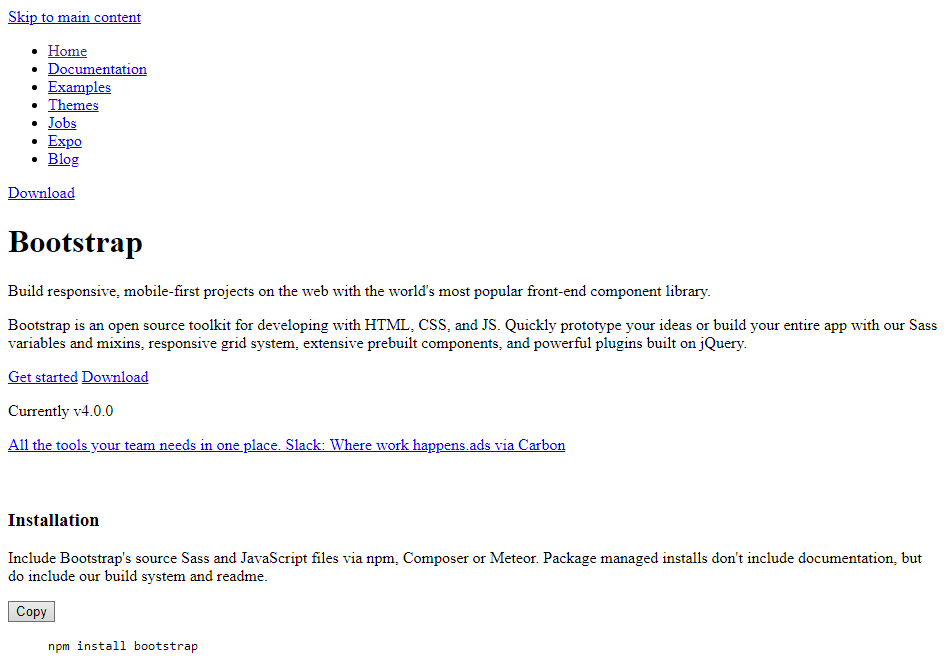
\includegraphics[width=0.75\textwidth]{figuras/withoutcss}
\begin{flushleft}
\flushleft{Fonte: Site do Bootstrap. Acesso em 9 de Abril de 2018.}
\end{flushleft}
\label{fig:withoutcss}
}
\end{figure}

O ponto ideal que queremos é onde renderizar a página com o CSS crítico necessário para estilizar a visualização principal, mas todo o CSS não crítico é carregado após a renderização inicial. Na Figura~\ref{fig:withcss} pode ser observada a aparência que deveria ser apresentada após o carregamento inicial de página.

\begin{figure}[th]
\centering{
\caption{Aparência Inicial Esperada.}
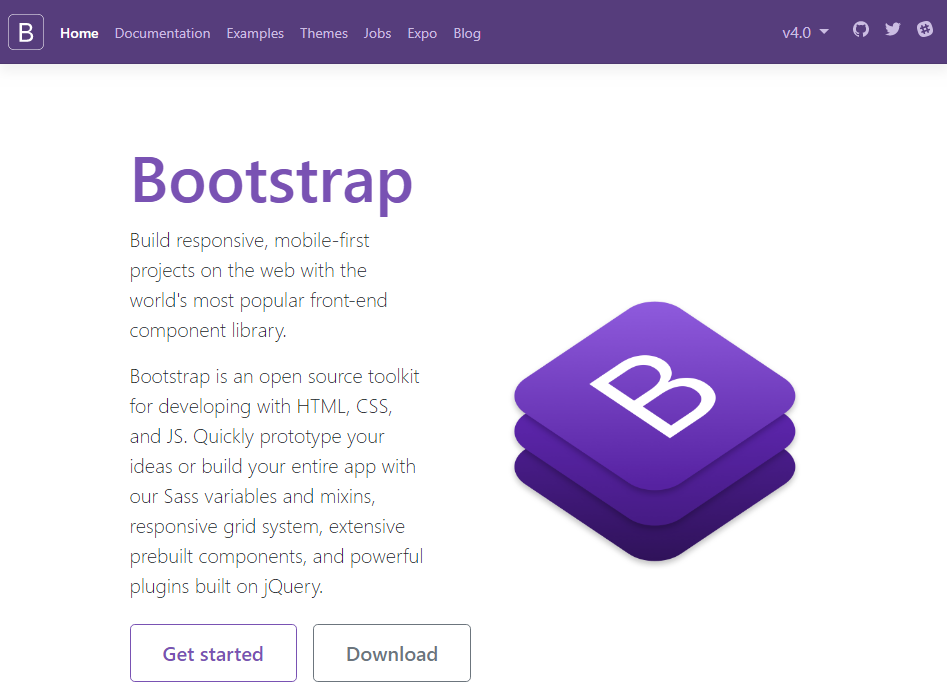
\includegraphics[width=0.75\textwidth]{figuras/withcss}
\begin{flushleft}
\flushleft{Fonte: Site do Bootstrap. Acesso em 9 de Abril de 2018.}
\end{flushleft}
\label{fig:withcss}
}
\end{figure}

Determinados componentes visuais, considerados críticos, devem aparecer de prontidão bem como suas regras de estilo. Todavia, componentes secundários que não representam impacto para a visualização inicial do documento não são necessários para a exibição imediata. Tendo isto em mente, é necessário isolar o CSS crítico do CSS não crítico. Para isto, são criadas duas folhas de estilo:~\texttt{critical.css} e \texttt{non\_critical.css}, que separam os estilos crítico do não-crítico, respectivamente. Suas importações podem ser realizadas através do elemento \texttt{<link>}, juntamente com \texttt{<script>} ou arquivo externo contendo JavaScript.

\begin{lstlisting}[label=criticalcss,caption=CSS Crítico.]
<!DOCTYPE html>
<html lang="pt-br">
    <head>
        <meta charset="utf-8">
        <title>Monografia</title>
        <link rel="stylesheet" href="critical.css">
    </head>
    <body>
        <script>
            require("non_critical.css");
        </script>
    </body>
</html>
\end{lstlisting}

O trecho de Código~\ref{criticalcss}, escrito em ES6 para fins didáticos, ilustra como acontece a importação de uma folha de estilos em cascata crítica. Através do cabeçalho do documento e um arquivo não crítico, importado por meio de código JavaScript no corpo do arquivo HTML. Estas duas importações fazem com que o arquivo crítico seja lido inicialmente, no momento que a página é carregada e, posteriormente, quando a árvore DOM estiver montada no documento. Sendo assim, quando o arquivo de \textit{script} for lido, o restante do estilo CSS é carregado junto ao documento também. É importante mencionar que o exemplo acima não funciona em navegadores atuais e, sua versão em ES5 foi omitida devido à grande extensão de linhas de código.

Como visto na Subseção~\ref{SubWebpack}, o \textit{Webpack} é responsável por resolver programaticamente diversas atividades. Ele pode ser útil com o auxílio de alguns \textit{plug-ins} para a identificação do CSS crítico automaticamente, visto que identificar manualmente pode ser uma tarefa árdua e repetitiva ao longo do período de desenvolvimento. Um destes \textit{plug-ins} é o~\texttt{critical}, disponível no NPM~\footnote{\textit{Node Package Manager} (NPM) é o maior gerenciador de pacotes para JavaScript, disponível em: https://www.npmjs.com/. Data de acesso: 10 de Abril de 2018.}. Este módulo em JavaScript é responsável pela leitura de um documento HTML, para, posteriormente identificar o CSS crítico através de uma renderização de página no servidor. Para isso, é utilizado o PhantomJS~\footnote{Phantom JS é um \textit{headless browser}, ou seja, um navegador que não renderiza as páginas. Ele apenas executa o código que está contido nas páginas, tornando-o uma ferramenta comum para um ambiente de integração contínua.}, outro módulo JavaScript disponível no NPM, que, por sua vez, extraias regras CSS aplicadas na página então renderizada pelo servidor com PhantomJS.

É importante ressaltar que esta solução descrita acima foi idealizada com base no cenário atual sob o protocolo HTTP/1.1, disponível na Subseção~\ref{SubHTTP}. Com o avanço do protocolo e a promessa de suportar multiplexação, o ideal é realizar requisições e respostas assíncronas e paralelas utilizando apenas uma conexão para baixar múltiplos arquivos. Isso pode fazer com que, através do protocolo HTTP/2 ou superior, seja possível obter primordialmente o código CSS crítico em uma modificação da técnica atual, através do uso da multiplexação em conjunto com \textit{Critical} CSS.

No Capítulo~\ref{Resultados}, são apresentados os resultados deste experimento. Com o intuito de validar a otimização em questão, espera-se obter um retorno satisfatório com base nas métricas utilizadas na execução do teste. Além disso, contém as descrições dos resultados dos experimentos.
%
%
%
\subsection{Reduzir o \textit{Payload}}
\label{SubPayload}

Em aplicações para rede de computadores e, principalmente voltadas para \textit{Web}, é inevitável deparar-se com o \textit{payload}~\footnote{\textit{Payload} refere-se à carga de uma transmissão de dados.}. Uma boa prática de desenvolvimento para aplicações \textit{Web} é tentar reduzir este volume de dados, uma vez que dados trafegam pela \textit{Web} entre aplicações distribuídas. Para isso, há diversas técnicas que podem ser utilizadas para reduzir o \textit{payload}.

Uma dessas técnicas é reduzir o número de requisições. Desenvolver serviços para Internet, pensando em baixas velocidades de conexão, bem como aplicando a estratégia do \textit{mobile first}~\footnote{\textit{Mobile First} é uma estratégia de desenvolvimento contrária ao histórico modelo de desenvolvimento de aplicações \textit{Web}, onde a versão móvel era tratada de forma secundária.}, são boas práticas para o desenvolvimento de aplicações \textit{Web}. Determinadas requisições podem ser irrelevantes por completo ou apresentar conteúdo parcialmente desnecessário. Por exemplo, ao realizar uma requisição HTTP com o verbo GET, os dados retornados são: \texttt{id}; \texttt{name}; \texttt{birthday}; \texttt{address}. Sendo que, esta requisição será utilizada apenas para popular um \texttt{<select>} que, por sua vez, necessita apenas de um atributo \texttt{value}, referenciando o valor selecionado de uma opção com um texto indicativo. Os dados necessários para popular este elemento HTML podem ser resumidos a dois: \texttt{id} e o dado exibido. Por exemplo, uma lista de usuários necessitaria de \texttt{id}~e~\texttt{name}, apenas.

Outra técnica comum, é o agrupamento de arquivos do mesmo tipo, como arquivos de \textit{script} e folhas de estilo, por exemplo. Apesar de aumentar o \textit{payload}, com a transferência de um arquivo único de \textit{bundle}, composto do agrupamento de todos os arquivos JavaScript, cujo o tamanho é a soma de todos os tamanhos dos arquivos aglomerados. A perda no aumento do \textit{payload} é compensada devido ao comportamento atual do protocolo HTTP/1.1, onde não há multiplexação e as requisições são síncronas, ou seja, um arquivo é enviado após o outro. As respostas, no melhor caso, retornam para o cliente com o mesmo custo de tempo de envio de um único arquivo aglomerado. Entretanto, podem ocorrer complicações em rede, tais como: Falha na entrega de um dos arquivos, causado pela perda de pacotes; Atraso na Rede, devido à latência ou congestionamento de fluxo; dentre outros problemas comuns em redes de computadores. Sendo assim, justifica-se a criação de um arquivo composto da união de vários outros para o envio.

Há também outro artificio que consiste em habilitar a compressão GZIP~\footnote{GZIP é um formato de compactação de arquivos, identificado pela extensão~\texttt{.gz}. Descrito na RFC 1952 por \citeonline{rfc1952}.}~no servidor. Esta técnica é suportada em todos os navegadores e servidores contemporâneos. Com o processo de compactação, todo o conteúdo textual (i.e. HTML, CSS, JS, etc) é comprimido antes de ser enviado para o cliente, contribuindo assim, para a diminuição do tráfego total em rede.

Em conjunto com a agregação de arquivos e redução do número de requisições, é importante também, comprimir os códigos gerados. Isto é, não basta escrever JavaScript elegante, bem documentado, organizado e padronizado. Estas características são agradáveis para se manter e manutenir, porém o navegador não entende linguagem humana não se importa com a organização do código. Enviar código padronizado via requisição HTTP para o lado cliente não acrescentará valor algum à performance do código. Para isto que deve-se utilizar um compressor de arquivos, por exemplo o módulo~\texttt{uglify-js}, disponível no NPM. Após agregar todos os \textit{scrips} em um único, tecnicamente, não há nada além de uma simples concatenação em um novo arquivo de \textit{script}. Com uma ferramenta de otimização, como o~\texttt{uglify-js}, o código agregado é processado e comprimido, a fim de diminuir o tamanho do arquivo gerado como saída. Neste processo, também chamado de \textit{minification}, os espaçamentos são removidos, assim como a indentação, a nomenclatura dos objetos e variáveis é renomeada para uma versão minificada baseada em escopo. Em outras palavras, uma variável chamada de~\texttt{option}~pode ser renomeada para apenas~\texttt{o}~e suas correspondentes dentro do escopo da função seguem o mesmo processo de maneira que não haja conflitos. Todo esse processo é realizado automaticamente e o resultado produz um arquivo de agregação comprimido e ilegível para linguagem humana, apresentando um menor número de caracteres.

Imagens também podem ser otimizadas, no formato~\texttt{.jpeg}, há uma série de metadados desnecessários. E no formato~\texttt{.png}, as paletas de cores são definidas, porém, também não são necessárias. Estas informações extra consomem alguns KB de memória a mais, que não representam importância para sua reprodução no cliente. Além desta otimização, é importante utilizar os atributos~\texttt{width}~e~\texttt{height}~para contribuir com os cálculos de dimensões realizados pelo navegador durante a renderização de página. Entretanto, não devem ser utilizados os mesmos atributos para redimensionar o tamanho das imagens importadas, devem ser declarados os tamanhos reais. Por exemplo, se uma imagem nas dimensões~\texttt{50px}~por~\texttt{50px}~for exibida, não deve-se importar uma imagem de tamanho superior e compensar a proporção com os atributos~\texttt{width}~e~\texttt{height}. O custo desta prática será a importação de uma imagem de tamanho superior e que não é utilizada, recomenda-se otimizar, também, a imagem em seu tamanho. 
 \chapter{RESULTADOS}
\label{Resultados}

Neste trabalho, são consideradas as tecnologias \textit{open-source} utilizadas para prover conteúdo na Internet, assim como, as boas práticas de desenvolvimento para aplicações \textit{Web} modernas apresentadas ao longo deste trabalho. São descritos neste capítulo, os resultados dos experimentos propostos no Capítulo~\ref{Proposta}, que são: Estratégias para a redução do \textit{payload}; Aplicação da técnica de \textit{Critical} CSS.

Os resultados esperados para os experimentos têm como objetivo reduzir o consumo de tempo na renderização de páginas e na resposta das requisições HTTP. Portanto, são utilizados os conceitos explanados e aplicados às boas práticas introduzidas ao longo desde trabalho.

A primeira aplicação prática, proposta na Subseção~\ref{SubCriticalCSS}, descreve a importância de haver separação do CSS crítico. Em outras palavras, há um conjunto de regras de formatação de página que são indispensáveis para a renderização inicial do documento HTML junto ao DOM. Em seguida, após a renderização do conteúdo crítico, os demais componentes visuais e folhas de estilo são requisitadas através de AJAX. Assim, o motor de renderização do navegador executa com mais fluidez a exibição da página devido à otimização no tamanho da árvore DOM a ser renderizada. Esta otimização é impulsionada pela aplicação da técnica de \textit{Critical} CSS. Entretanto, os resultados não contêm dados de requisições realizadas após a renderização inicial. Na Figura~\ref{fig:withoutcritical}, pode-se observar o gráfico de desempenho de renderização antes da técnica ser implementada.

\begin{figure}[th]
\centering{
\caption{Desempenho antes do \textit{Critical} CSS.}
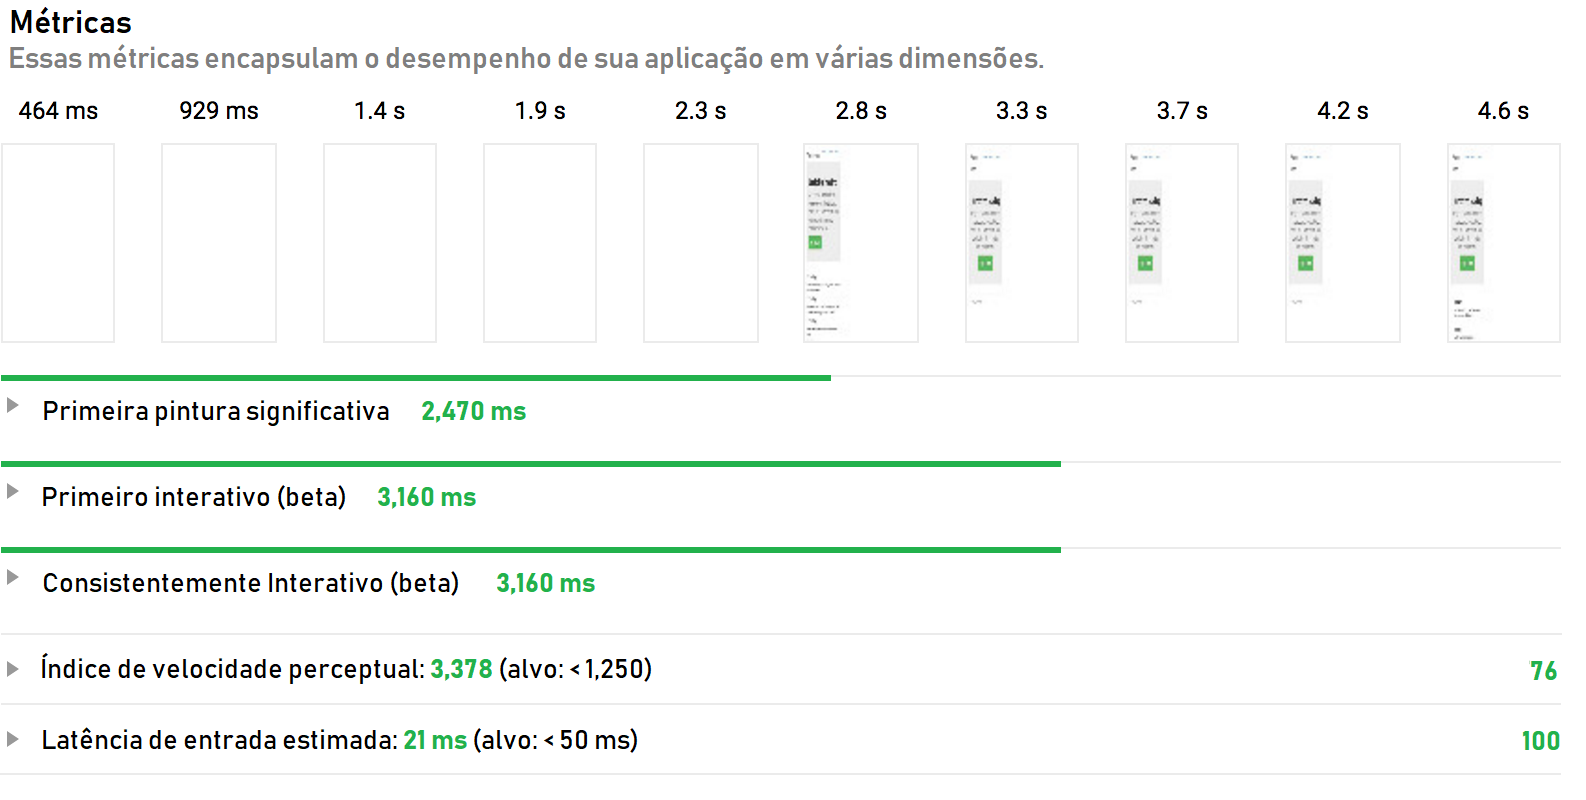
\includegraphics[width=0.75\textwidth]{figuras/critical_css_before}
\begin{flushleft}
\flushleft{Fonte: Gerado no \textit{Lighthouse}, por Anthony Gore.}
\end{flushleft}
\label{fig:withoutcritical}
}
\end{figure}

O desempenho da renderização, é medido através da ferramenta \textit{Lighthouse}~\footnote{Disponível em: https://goo.gl/H8EpEJ. Data de Acesso: 18 de Abril de 2018.}, uma extensão para navegador, automatizada e de código fonte aberto. A \textit{Lighthouse} é desenvolvida e mantida pela mesma equipe responsável pelo Google Chrome, e a mesma é utilizada para auditar a qualidade de renderização das páginas \textit{Web}. Através da utilização desta ferramenta, foi gerado um relatório, apresentado na Figura~\ref{fig:withoutcritical}, que lista métricas utilizadas para medir o desempenho da renderização da página \textit{Web}, tais como: Primeira pintura significativa~\footnote{Tempo necessário para que o conteúdo principal de uma página seja visível.}; Eventos de interação~\footnote{Tempo em que a página torna-se interativa.}; Índice de velocidade perceptual~\footnote{Velocidade com que o conteúdo de uma página é visivelmente preenchida.} e Latência de entrada estimada~\footnote{Tempo, em milissegundos, que a aplicação necessita para responder a entrada no usuário.}. Todavia, apenas o comportamento da primeira pintura significativa é avaliada, devido ao impacto causado pela técnica testada sobre a métrica. Em outras palavras, devido ao tempo que leva até que o usuário possa perceber conteúdo na página. Na Figura~\ref{fig:withcritical}, pode-se perceber a melhoria do desempenho após o isolamento do CSS crítico do restante da folha de estilos em cascata.

\begin{figure}[th]
\centering{
\caption{Desempenho depois do \textit{Critical} CSS.}
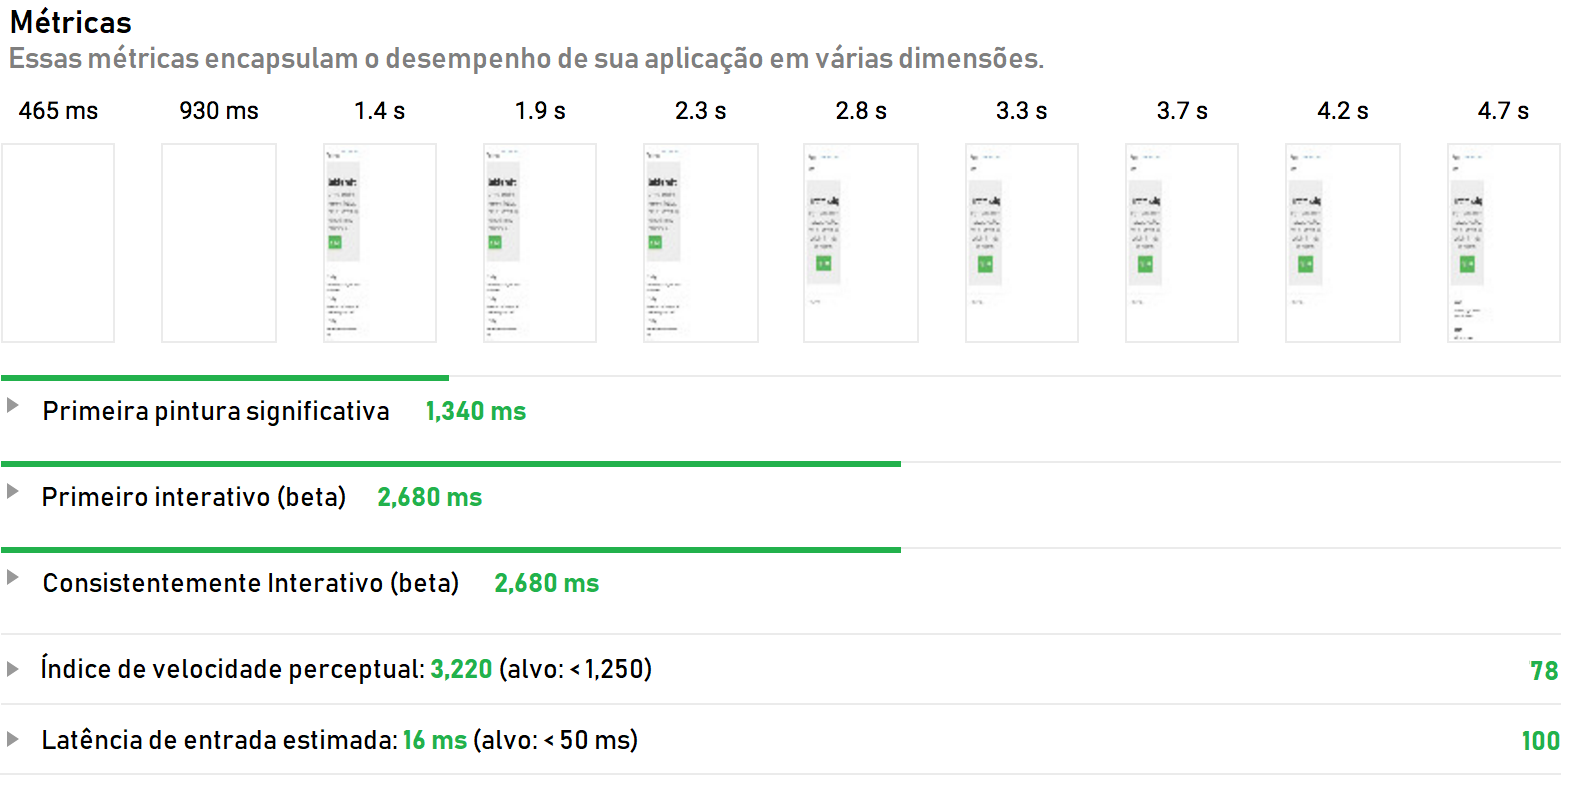
\includegraphics[width=0.75\textwidth]{figuras/critical_css_after}
\begin{flushleft}
\flushleft{Fonte: Gerado no \textit{Lighthouse}, por Anthony Gore.}
\end{flushleft}
\label{fig:withcritical}
}
\end{figure}

Logo após a implementação da técnica de \textit{Critical} CSS, é possível observar uma diminuição significativa no tempo necessário para a primeira pintura de página. Esta redução, foi de, aproximadamente, 54\% em relação ao mesmo resultado antes da aplicação da técnica. É perceptível tal otimização, pois o tempo necessários para a apresentação primeiro efeito visual foi reduzido de 2470ms para 1340ms. Esta melhoria, proposta por Anthony Gore, reduziu, também, o tempo necessário para a liberação dos eventos de interação na página, que podem ser manipulados pelo usuário ou por animações. Além destes eventos de interatividade, as métricas de Latência de entrada estimada e Índice de velocidade perceptual, sofreram variações. Entretanto, não há melhora significativa, para estas últimas métricas. Porém a aplicação da técnica não compromete o desempenho das outras métricas auditadas.

Os resultados foram obtidos a partir de um documento HTML com a adição de uma biblioteca CSS (\textit{Bootstrap}), aproximadamente 217 \textit{kilobytes} (que é um tamanho considerável para uma página simples de testes). A escolha da biblioteca é arbitrária e pode ser substituída por qualquer código CSS. Outras métricas podem ser obtidas a partir da extensão \textit{Lighthouse}, porém, não agregam valor à proposta inicial deste trabalho. Devido a este fato, novos resultados não foram adicionados, restando apenas cinco otimizações que culminaram em sucesso após a aplicação da técnica.

O Capítulo~\ref{Proposta}, também apresenta outra otimização importante, que é a redução do \textit{payload}. Essa estratégia utiliza um conjunto de técnicas voltadas à otimização do desempenho de renderização da página, que incluem: Redução do número de requisições realizadas; Redução da quantidade de dados enviados nas requisições; Aglomeração de arquivos do mesmo tipo; Compressão GZIP pelo servidor; Compressão do código gerado.

O ambiente de testes é fornecido pela Lux Teams~\footnote{Disponível em: https://app.teamslux.com/. Data de Acesso: 12 de Abril de 2018.}, um sistema integrado de gerência de reuniões, acompanhamento de projetos e tarefas. Bem como, a utilização do \textit{Firefox Developer Edition}~\footnote{Disponível em: https://www.mozilla.org/pt-BR/firefox/channel/desktop/. Data de Acesso: 18 de Abril de 2018.}, um navegador criado para atender as necessidades dos desenvolvedores \textit{Web} em seus testes. Os experimentos propostos, utilizam duas versões do sistema, que são: Versão 1.0, desenvolvida sem \textit{code-pattern} e não otimizada; Versão atual (2.1), apesar de não concluída, esta versão, está em fase avançada e os resultados de performance não são interferidos, visto que as métricas utilizadas estão estáveis. Além deste fato, a nova versão utilizou (desde o início do desenvolvimento), \textit{code-pattern} e otimizações. A seguir, é detalhada a redução do \textit{payload} nesta comparação.

\begin{figure}[th]
\centering{
\caption{\textit{Payload} antes da otimização.}
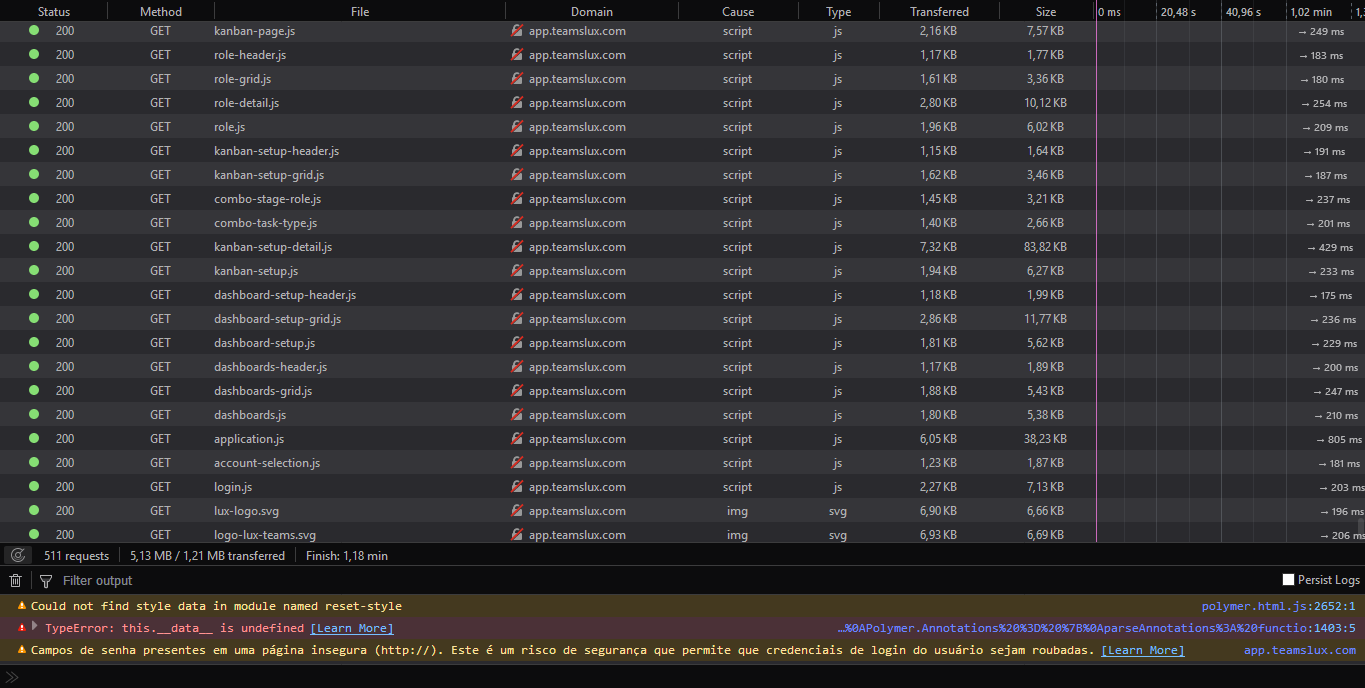
\includegraphics[width=1\textwidth]{figuras/oldlux.png}
\begin{flushleft}
\flushleft{Fonte: Disponibilizado pelo Autor.}
\end{flushleft}
\label{fig:oldlux}
}
\end{figure}

Nas Figuras~\ref{fig:oldlux}~e~\ref{fig:newlux}, podem ser observadas, o número de requisições realizadas a partir da entrada com credenciais no sistema (\textit{Login}) até o carregamento completo da tela principal. Além do \textit{payload} e o tempo de transferência necessário para o recebimento de todas as requisições. Os experimentos foram realizados múltiplas vezes para obter-se um resultado justo, com base na média. Além disso, a leitura de desempenho foi medida em horários de menor pico, de forma que, a interferência de rede seja mínima para o resultado final do teste realizado.

O \textit{payload} antes da otimização, na Figura~\ref{fig:oldlux}, possuía 5,13 \textit{megabytes} correspondentes com as 511 requisições disparadas. O tempo de resposta de todas as requisições durou aproximadamente 71 segundos (1,18 minuto), o que é lento. Após implementar as modificações propostas para a redução do \textit{payload}, pode-se observar na Figura~\ref{fig:newlux}~o resultado desta otimização.

\begin{figure}[th]
\centering{
\caption{\textit{Payload} depois da otimização.}
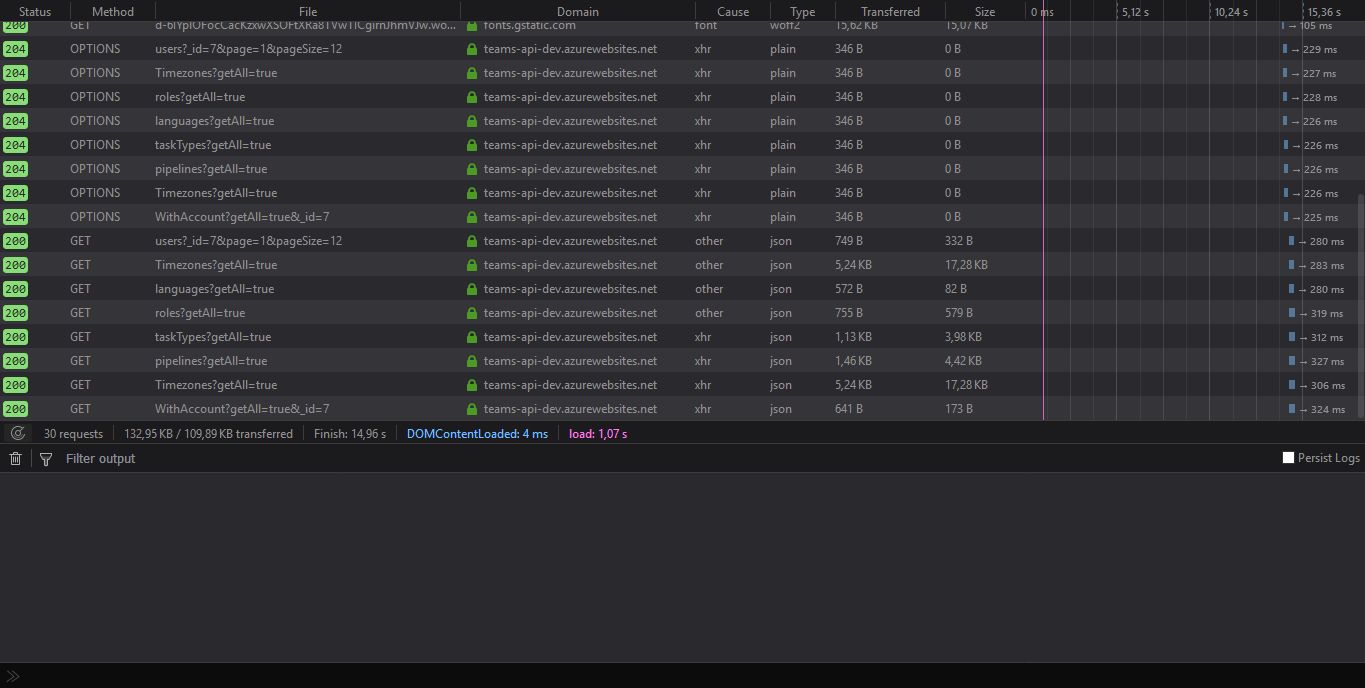
\includegraphics[width=1\textwidth]{figuras/newlux.png}
\begin{flushleft}
\flushleft{Fonte: Disponibilizado pelo Autor.}
\end{flushleft}
\label{fig:newlux}
}
\end{figure}

Ao final de todas as implementações, observa-se uma redução significativa em todas as métricas avaliadas na Figura~\ref{fig:newlux}. Antes da otimização, haviam 511 requisições. Já após a otimização, esse número foi reduzido para 30 requisições, 5.87\% do número total de requisições. Além da diminuição da duração total da requisição para apenas 15 segundos, 21.1\% do tempo total de aproximadamente 71 segundos. Esta redução pode ser explicada pela necessidade de consumir o recurso da API REST apenas quando solicitado. Em outras palavras, foi observado que, várias requisições poderiam ser solicitadas por demanda, não havendo necessidade em requisitar todo o conteúdo após a entrada no sistema, o que impactava, inclusive, o carregamento da página inicial. Além desta métrica, o tamanho de dados a serem transferidos, bem como o tempo necessário para todas as requisições serem finalizadas foram reduzidos. Este comportamento deve-se principalmente à redução do número total de requisições. É pertinente observar que ao utilizar-se da Internet para trafegar os dados, a Aplicação \textit{Web} está sucessível a erros e complicações de rede ligados diretamente ao modo que os protocolos que compõem a Internet operam. Isto é, lentidão na entrega causadas por congestionamentos de rede, perca de pacotes, latência na entrega devido a múltiplos saltos, tamanho das requisições e respostas. Todas essas problemáticas são inevitáveis e estão presentes em qualquer rede de computadores convencional ao modelo TCP/IP que é difundido por toda Internet. Entretanto, otimizações podem ser aplicadas, assim como neste trabalho, a fim de diminuir o impacto de um eventual problema de rede. Sendo assim, o usuário final observará um menor atraso na exibição de dados, o que contribui diretamente para melhorar a usabilidade da aplicação em questão. 
 \chapter{CONCLUSÃO}
\label{Conclusao}

Com a rápida evolução de soluções \textit{Web}, surgem também diversas formas de desenvolvimento. No entanto, é importante definir quais são as melhores ferramentas e estratégias para alcançar os objetivos de uma aplicação \textit{Web} de qualidade. Levando isso em consideração, este trabalho apresentou um conjunto de técnicas amplamente utilizadas para a otimização de aplicações \textit{Web}, exemplificando através de \textit{scripts} didáticos e de um sistema real em funcionamento.

A partir dos resultados, conclui-se neste trabalho que, a aplicação de boas práticas de programação durante o período de desenvolvimento, influenciam diretamente na performance da aplicação. Como é possível perceber nesta proposta, as otimizações descritas, quando implementadas corretamente, produzem significativos resultados. Esta percepção se faz possível ao utilizar técnicas de potencialização da aplicação focadas em fluidez e experiência do usuário.

\section{Trabalhos Futuros}
\label{TrabalhosFuturos}

Podem ser apresentados, na sequência deste trabalho, a introdução de boas práticas para o desenvolvimento de aplicações \textit{Web} utilizando novos conceitos referente às tecnologias citadas neste trabalho. São exemplos de trabalhos futuros: Técnicas de otimização de código e obtenção de maior desempenho na execução, além da abordagem de novos recursos para as futuras versões da HTML, da CSS e do JS; Adaptação na estrutura e arquitetura da aplicação para se obter o máximo de integração com as novas versões dos protocolos para transferência de arquivos, que causam impacto direto no desempenho das aplicações; Abordagem e inclusão de modelos e conceitos de aplicações \textit{Web}, tais como \textit{Single Page Application} (SPA) e \textit{Progressive Web Apps} (PWA); Integração com novas tecnologias, como \textit{Web Assembly}. 

% ELEMENTOS PÓS-TEXTUAIS
\postextual
% Referências bibliográficas
\bibliography{abntex2-modelo-references} 
%\begin{apendicesenv}
	\partapendices
	\chapter*{APÊNDICE A - TÍTULO}
	\lipsum[5]
	\chapter*{APÊNDICE B - TÍTULO}
	\lipsum[5]
\end{apendicesenv}
 
%\begin{anexosenv}
%Imprime uma página indicando o início dos anexos
	\partanexos
	\chapter*{ANEXO A - TÍTULO}
	\lipsum[10]
	\chapter*{ANEXO B - TÍTULO}
	\lipsum[10]
\end{anexosenv}
 


% INDICE REMISSIVO
%\printindex

\end{document}

